\documentclass[
	openany,
	% -- opções da classe memoir --
	12pt,				% tamanho da fonte
   % openright,
	%twoside,
    oneside,
    % para impressão em verso e anverso. Oposto a oneside
	a4paper,			% tamanho do papel. 
	brazil]{abntex2}

% ---
% Pacotes básicos 
% ---

\usepackage{fontspec}
\setmainfont{Arial}

\usepackage[utf8]{inputenc}		% Codificacao do documento (conversão automática dos acentos)
\usepackage{indentfirst}		% Indenta o primeiro parágrafo de cada seção.
\usepackage{color}				% Controle das cores
\usepackage{graphicx}			% Inclusão de gráficos
\usepackage{microtype} 			% para melhorias de justificação
\usepackage{multicol}			% multiplas colunas no texto
\usepackage{subcaption}
\usepackage{caption}
\usepackage{float}
\usepackage{amsmath}
\usepackage{amssymb}
\usepackage{amsthm}
\usepackage{lipsum}
\usepackage{blindtext}


% ---
% ---
% Pacotes de citações
% ---
\usepackage[brazilian]{backref}	 % Paginas com as citações na bibl
\usepackage[alf]{abntex2cite}	% Citações padrão ABNT

% --- 
% CONFIGURAÇÕES DE PACOTES
% --- 

% ---
% Configurações do pacote backref
% Usado sem a opção hyperpageref de backref
\renewcommand{\backrefpagesname}{Citado na(s) página(s):~}
% Texto padrão antes do número das páginas
\renewcommand{\backref}{}
% Define os textos da citação
\renewcommand*{\backrefalt}[4]{
	\ifcase #1 %
		Nenhuma citação no texto.%
	\or
		Citado na página #2.%
	\else
		Citado #1 vezes nas páginas #2.%
	\fi}%
% ---

% ---
% Informações de dados para CAPA e FOLHA DE ROSTO
% ---
\titulo{What Weee Are - Jogo eletrônico para educação de reciclagem de resíduos eletrônicos}
\autor{Richard da Cruz Lopes}
\local{Santo André}
\data{2023}
\orientador{Prof. Dr. André Luiz Brandão}

\instituicao{%
	Fundação Universidade Federal do ABC -- UFABC
  	\par
  	Centro de Matemática, Computação e Cognição -- CMCC
    \par
  	Curso de Bacharelado em Ciência da Computação
}

\tipotrabalho{Projeto de Graduação em Computação}
% O preambulo deve conter o tipo do trabalho, o objetivo, 
% o nome da instituição e a área de concentração 
\preambulo{Monografia  apresentada  ao  Centro  de  Matemática, Computação  e  Cognição  -  CMCC/UFABC - como parte dos requisitos necessários à obtenção do título de Bacharel em Ciência da Computação}
% ---


% ---
% Configurações de aparência do PDF final

% alterando o aspecto da cor azul
\definecolor{blue}{RGB}{41,5,195}

% informações do PDF
\makeatletter
\hypersetup{
     	%pagebackref=true,
		pdftitle={\@title}, 
		pdfauthor={\@author},
    	pdfsubject={\imprimirpreambulo},
	    pdfcreator={LaTeX with abnTeX2},
		colorlinks=true,       		% false: boxed links; true: colored links
    	linkcolor=blue,          	% color of internal links
    	citecolor=blue,        		% color of links to bibliography
    	filecolor=magenta,      		% color of file links
		urlcolor=blue,
		bookmarksdepth=4,
        draft=false
}
\makeatother
% --- 

% --- 
% Espaçamentos entre linhas e parágrafos 
% --- 

% O tamanho do parágrafo é dado por:
\setlength{\parindent}{1.3cm}

% Controle do espaçamento entre um parágrafo e outro:
\setlength{\parskip}{0.2cm}  % tente também \onelineskip

% ---
% compila o indice
% ---
\makeindex
% ---

% Requisitos mínimos PGC I :
%(I) Dados de identificação           OK Feito
%(II) Introdução                      OK Feito
%(III) Justificativa                  OK Feito
%(IV) Objetivos                       OK Feito
%(V) Metodologia                      DESCREVER TELAS         
%(VI) Cronograma                      REMOVER        
%(VII) Referências Bibliográficas     OK Feito

% ----
% Início do documento
% ----
\begin{document}

% Seleciona o idioma do documento (conforme pacotes do babel)
%\selectlanguage{english}
\selectlanguage{brazil}

% Retira espaço extra obsoleto entre as frases.
\frenchspacing 

% ----------------------------------------------------------
% ELEMENTOS PRÉ-TEXTUAIS
% ----------------------------------------------------------
% \pretextual
%\begin{figure}[h]
%\centering % este comando é usado para centralizar a figura
%\includegraphics[width=7cm]{figuras/logo_ufrpe_horizontal.png}\\
%\end{figure}

% \begin{figure}[ht]
% \centering
% \begin{minipage}[b]{0.45\textwidth}
% \includegraphics[height=3cm]{figuras/logo_ufrpe_horizontal.png}
% \end{minipage}
% \qquad
% \begin{minipage}[b]{0.45\textwidth}
% \includegraphics[height=2.5cm]{figuras/logo_bsi.pdf}
% \end{minipage}
% \end{figure}

%\begin{minipage}[t]{1\textwidth}
%	\begin{figure}[ht]
%		\includegraphics[height=3cm]{figuras/logo_ufrpe_horizontal.png}
%		\hspace{4.5cm}
%   	\includegraphics[height=2.5cm]{figuras/logo_bsi.pdf}
%	\end{figure}    
%\end{minipage}

% ---
% Capa
% ---
%\imprimircapa
% ---
% ---
% Folha de rosto
% (o * indica que haverá a ficha bibliográfica)
% ---
\imprimirfolhaderosto
% ---

% dedicatoria
%\begin{dedicatoria}
   \vspace*{\fill}
   \centering
   \noindent
   \textit{À \ldots\\} \vspace*{\fill}
\end{dedicatoria}

% agradecimentos
\begin{agradecimentos}
\indent Agradeço aos meus pais, por terem me dado oportunidade de estudar;

\indent Agradeço ao meu orientador, André Luiz Brandão, por todos os conselhos, papos, trocas de ideias e além de tudo pela paciência e ajuda nesse período.
\\
\indent Aos meus amigos Carlos, Willian e todos os outros por estarem presentes na minha vida durante todos estes anos.

\indent Aos professores Jesus Mena, Emílio Francesquini, Carla Lopes, Isidro. Por serem inspiradores aos seus alunos.

\indent À UFABC pela jornada até aqui.

\end{agradecimentos}

% epigrafe
%\begin{epigrafe}
    \vspace*{\fill}
	\begin{flushright}
		\textit{``A persistência é o caminho do êxito.'' \\
		(Charles Chaplin)}
	\end{flushright}
\end{epigrafe}

% resumo e abstract

% ---
% RESUMOS
% ---

% RESUMO em português
\setlength{\absparsep}{18pt} % ajusta o espaçamento dos parágrafos do resumo
\begin{resumo}

O trabalho apresenta o desenvolvimento de um jogo eletrônico educativo voltado para a educação em reciclagem de resíduos eletrônicos. O objetivo principal é abordar a problemática do descarte inadequado do lixo eletrônico e promover a conscientização sobre a importância da reciclagem desses materiais. O jogo foi desenvolvido utilizando o motor gráfico Unity e a linguagem de programação C\#.

O estudo aborda a eficácia dos jogos cognitivos na promoção da motivação, envolvimento e engajamento dos alunos, bem como no desenvolvimento de habilidades e conhecimentos. Além disso, explora a interação proporcionada pelos jogos e seu papel crucial na aquisição de conhecimento. O trabalho também destaca o impacto socioambiental causado pela falta de gerenciamento de lixo eletrônico e as oportunidades e desafios associados à gamificação em contextos educacionais.

Como resultado, o jogo "What Weee Are" foi apresentado a estudantes do ensino fundamental e médio, gerando um maior interesse e envolvimento dos alunos no tema da reciclagem de materiais eletrônicos. A análise hierárquica de tarefas foi utilizada para desenvolver as mecânicas e a progressão do jogo.

 \textbf{Palavras-chaves}: lixo eletrônico, jogo, jogo educativo, computação, ecologia, resíduo eletrônico, REEE, e-lixo.
\end{resumo}

% ABSTRACT in english
\begin{resumo}[Abstract]
 \begin{otherlanguage*}{english}
The paper presents the development of an educational electronic game focused on electronic waste recycling education. The main objective is to address the problem of inadequate disposal of electronic waste and promote awareness of the importance of recycling these materials. The game was developed using the Unity graphics engine and the C\# programming language.

The study addresses the effectiveness of cognitive games in promoting student motivation, engagement, and involvement, as well as in the development of skills and knowledge. Additionally, it explores the interaction provided by games and their crucial role in knowledge acquisition. The paper also highlights the socio-environmental impact caused by the lack of electronic waste management and the opportunities and challenges associated with gamification in educational contexts.

As a result, the game "What Weee Are" was presented to elementary and high school students, generating greater interest and engagement among students in the topic of electronic materials recycling. The hierarchical task analysis was used to develop the mechanics and progression of the game.
   \vspace{\onelineskip}
 
   \noindent 
   \textbf{Keywords}: electronic waste, game, educational game, computing, ecology, electronic waste, WEEE, e-waste.
 \end{otherlanguage*}
\end{resumo}

% Lista de ilustrações
\pdfbookmark[0]{\listfigurename}{lof}
\listoffigures*
\cleardoublepage

% Lista de ilustrações
\pdfbookmark[0]{\listoftables}{lot}
\listoftables*
\cleardoublepage

% ---
% inserir o sumario
% ---
\pdfbookmark[0]{\contentsname}{toc}
\tableofcontents*
\cleardoublepage
% ---



% ----------------------------------------------------------
% ELEMENTOS TEXTUAIS
% ----------------------------------------------------------
\textual

% ----------------------------------------------------------
% inclusao das secoes do texto
% ----------------------------------------------------------
\chapter{Introdução}

O Brasil, como membro da Organização das Nações Unidas (ONU), comprometeu-se numa agenda a concluir dezessete Objetivos de Desenvolvimento Sustentável~\cite{odsbrasil} até 2030. Jogos são uma forma de entretenimento popular e amplamente acessível, que pode envolver jogadores em tarefas desafiadoras e educacionais. Quando usados de maneira estratégica, podem ser ferramentas poderosas para engajar a população em causas importantes, como a promoção dos Objetivos de Desenvolvimento Sustentável (ODS) estabelecidos pela ONU. Os jogos podem transmitir informações de forma interativa e envolvente, permitindo que os jogadores sejam incentivados a aprender sobre qualquer questão. Neste sentido, jogos podem servir como ferramentas de interação para atingir uma parcela da população e colaborar para o alcance desses objetivos. Além disso, campanhas conscientizadoras por meio de jogos podem incentivar comportamentos mais sustentáveis~\cite{joseamericonetoGameOds}.

\par
Visto que os problemas ambientais podem afetar diretamente os objetivos de desenvolvimento social, é importante considerar que a atualidade conta com um acelerado avanço tecnológico combinado com o descarte muitas vezes incorreto dos materiais eletrônicos produzidos, bem como dos resíduos gerados. Como consequência, essas questões nem sempre recebem a atenção que merecem. Existem várias razões pelas quais essas questões ambientais muitas vezes não recebem a atenção necessária. Algumas dessas razões incluem falta de conscientização sobre a importância do meio ambiente, falta de regulamentações e políticas públicas efetivas, interesses econômicos em conflito com a proteção ambiental, falta de recursos financeiros para investimentos em sustentabilidade, entre outras. Além disso, muitas vezes ações ambientalmente corretas requerem mudanças de comportamento e hábitos, o que pode ser difícil de implementar em larga escala.
Considerando que os recursos empregados na produção de produtos eletrônicos são limitados e que seu descarte inadequado pode provocar a contaminação de solos e lençóis freáticos \cite{eWasteContamination}, a problemática em questão se alinha com os Objetivos de Desenvolvimento Sustentável (ODS) da Organização das Nações Unidas (ONU), que buscam abordar os desafios ambientais globais e alcançar um futuro mais sustentável até 2030. Nesse sentido, a gestão adequada de resíduos eletrônicos é fundamental para garantir a preservação do meio ambiente e a promoção de um desenvolvimento sustentável em escala global.
\par
Podemos utilizar jogos sérios educativos como uma ferramenta de aprendizado para conscientização e informação sobre assuntos como o descarte de materiais eletrônicos. Além disso, esses jogos permitem apresentar sistemas complexos de um modo dinâmico, ampliando a compreensão acerca de conteúdos. Eles não se restringem a leituras ou a assistir, mas também permitem interagir, proporcionando um papel ativo ao jogador, o que os torna uma excelente forma de aprendizado. \cite{Vasconcellos_Carvalho_Barreto_Atella_2017}
\par

Pela ótica da Interação Humano-Computador, o processo de design pode auxiliar na análise da situação, síntese da intervenção e avaliação da nova situação. Temos que:
\begin{itemize}
    \item A análise da situação evidencia o compromisso assumido pelo Brasil em relação aos dezessete Objetivos de Desenvolvimento Sustentável estabelecidos pela ONU, os quais devem ser alcançados até o ano de 2030. Entretanto, há um problema ecológico preocupante relacionado à poluição gerada pelos materiais eletrônicos que tem sido negligenciado e merece atenção imediata. É importante salientar que tal problemática não foi mencionada na agenda da COP26, conforme afirmado por \cite{skelton_2021} . Dessa forma, faz-se necessário que sejam adotadas medidas efetivas para o controle e redução desse tipo de poluição, a fim de garantir o cumprimento dos objetivos estabelecidos pela ONU e a preservação do meio ambiente para as gerações futuras.
    \item A presente intervenção tem como objetivo desenvolver uma ferramenta lúdica que aborde questões climáticas e de reciclagem de materiais eletrônicos, conhecido como WEEE (\textit{Waste Electrical and Electronic Equipment}). Tal ferramenta é um jogo educativo, intitulado What Weee Are, que busca disseminar o conhecimento acerca das consequências do descarte inadequado de materiais eletrônicos e sensibilizar o público infantil sobre a importância da reciclagem e do consumo consciente. Dessa forma, espera-se contribuir para a formação de uma geração mais consciente e comprometida com a preservação ambiental.
\end{itemize}
\begin{figure}[h]
    \centering
    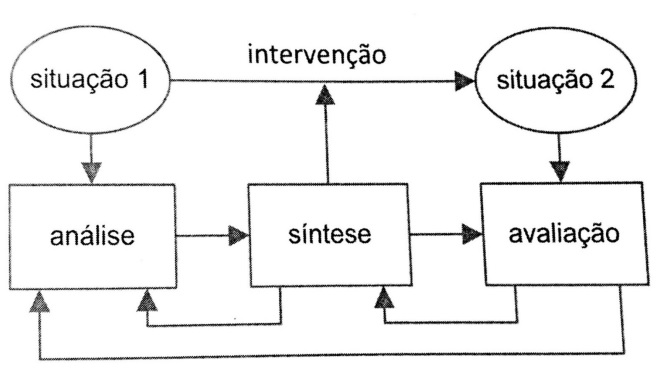
\includegraphics[width=\textwidth]{figuras/intervencao.jpg}
    \caption{Fluxograma do modelo de Análise de Situação e Síntese da Intervenção.}
    \label{fig_intervencao}
\end{figure}
\par
Este trabalho envolveu a co-criação com Alessio De Marchi. Alessio concebeu a ideia inicial do jogo e contribuiu para o design de algumas mecânicas e interações, bem como para a narrativa abordada pelo jogo. Além disso, ele forneceu os materiais artísticos necessários para a execução do jogo, conhecidos como \textit{Assets}. Durante a primeira reunião síncrona, foi definido o andamento do jogo, a quantidade de cenários presentes e quais seriam os inimigos presentes até aquele estágio. Posteriormente, outra reunião foi realizada para revisar o progresso e discutir possibilidades de adições ao jogo, como a inclusão de diálogos. Durante os meses seguintes, houve trocas de e-mails para atualizações do desenvolvimento e sugestões de novas adições ao produto final, a partir dos conceitos iniciais propostos por Alessio. Esses conceitos incluíam a possibilidade de melhorar as habilidades do personagem e a coleta de materiais, bem como a inclusão de laboratórios de desmonte e montagem nos cenários, conforme mencionado em documentos iniciais.
\par
%TODO
Cocriação é uma iniciativa de gestão, ou forma de estratégia econômica, que reúne diferentes partes (por exemplo, uma empresa e um grupo de clientes), a fim de produzir conjuntamente um resultado mutuamente valorizado \cite{PRAHALAD20045}. Podendo ser utilizado na frente do desenvolvimento de software, dentro de si, no desenvolvimento de jogos digitais, jogos digitais voltados para educação e saúde \cite{IHC_Estendido}, democraticamente inserindo pluralmente pessoas de amplas competências no desenvolvimento de um projeto complexo, "Participantes que jamais imaginaram-se usando um computador criaram seus jogos digitais. Participantes inicialmente inseguros com o uso de computadores começaram a ensinar outras pessoas a usarem para que pudessem jogar seus projetos." \cite{IHC_Estendido}.
\par
Um jogo chamado Par Tribus, desenvolvido por meio da cocriação, no Reino Unido, pela empresa Denki, por meio de\textit{feedbacks} de potenciais jogadores, minimizando riscos ouvindo-os, driblando um desperdício de material humano, de desenvolvimento técnico e evitar que apenas no final do desenvolvimento do jogo descobrir que ninguém o quer, isso ajudou a empresa a ter previsibilidade do seu produto \cite{lowthorpe2013stop}.
\par
Cocriação não é pedir aos clientes o que eles querem, mas sim, busca por \textit{feedback} criativo para soluções, para fazer uma entrega de valor agregado com o produto final e de participação conjunta, além de trazer uma visão sem viés técnico que desenvolvedores possuem. A multidisciplinaridade consegue se beneficiar da cocriação, pois consegue por meio da participação conjunta, trazer perspectivas plurais à concepção do que está sendo trabalhado, trazendo interações mais igualitárias e pelos participantes \cite{rock2018multidisciplinary}
\par
%TODO
Pela falta na literatura brasileira, de um trabalho que aborde o desenvolvimento de um jogo educacional que trata do problema causado pelos resíduos de materiais eletrônicos descartados de maneira incorreta, assim surge a proposta de um jogo digital, chamado What Weee Are, a ser inserido e apresentado à crianças e adolescentes em idade escolar, para auxiliar na aprendizagem, com a intenção de apresentar o risco da má gestão de resíduos de materiais eletrônicos, da falta de reciclagem. Jogos educacionais são uma ferramenta que pode ser utilizada para apresentação de conceitos de uma maneira interativa e lúdica às pessoas, além de ter sido identificado benefícios cognitivos e comportamentais do uso desta ferramenta \cite{gameUseOnSchool}, além de gerar curiosidade e interesse por parte daqueles que estão sendo apresentados, neste caso, crianças e adolescentes em idade escolar. \cite{savi2008jogos} 
\par
%TODO
What Weee Are é um projeto multimídia, um jogo eletrônico que aborda os desperdício de recursos de nossa sociedade, a ideia é que o jogo seja capaz de ser usado como uma ferramenta educacional a ser utilizada pelos professores, capaz de motivar o interesse dos alunos à reciclagem de materiais eletrônicos, um dos problemas atuais de nossa sociedade. Utilizar um jogo como ferramenta de educação já foi apresentado como viável e devemos aproveitar as oportunidades que o atual mundo tecnológico nos apresenta \cite{gameUseOnSchool}


\section{Justificativa}
\label{Justificativa}
Contudo, a partir de tudo isso, com os Objetivos de Desenvolvimento Sustentáveis da ONU para o Brasil \cite{odsbrasil}, e de como a educação é uma espaço onde existe a importância de levar conteúdos de impacto para o futuro e de como jogos sérios podem ser uma ótima ferramenta para ser utilizada no ensino e apresentação de conteúdos \cite{gameUseOnSchool}, de uma maneira mais dinâmica e ativa por parte dos alunos \cite{savi2008jogos}, e utilizando conceitos de Interação Humano-Computador para a concepção e desenvolvimento do projeto interativo \cite{IHC_Estendido}, por meio do fluxo de análise, síntese da intervenção e avaliação, da cocriação como ferramenta de desenvolvimento conjunto entre partes \cite{lowthorpe2013stop}. What Weee Are, propõe correlacionar estes três pontos junto com o problema dos resíduos de materiais eletrônicos no planeta.

\section{Objetivos}
\label{Objetivos}

\subsection{Objetivos Gerais}
% Objetivo geral é aplicar o co-design para o desenvolvimento de um sistema educativo
O objetivo do projeto acadêmico "What Weee Are" é desenvolver um jogo educativo utilizando técnicas de programação, boas práticas e estruturas de dados adequadas, com foco na conscientização sobre a importância da reciclagem de resíduos eletrônicos. O projeto também utiliza o co-design para permitir a participação dos usuários finais no processo de criação do sistema interativo e criar um produto que atenda às suas necessidades e expectativas.

O jogo será aplicado em escolas como uma ferramenta educativa para conscientizar os estudantes sobre a importância da reciclagem de resíduos eletrônicos e incentivar a sua participação nesse processo. Através da aplicação de conceitos de Interação Humano-Computador, o jogo será desenvolvido de forma clara e organizada para facilitar a manutenção e expansão futura do projeto.

\subsection{Objetivos Específicos}
No projeto What Weee Are, por meio da utilização do motor gráfico de desenvolvimento de jogos Unity como ferramenta de criação de jogos. O objetivo é permitir que os usuários interajam com o projeto de forma intuitiva e envolvente.

Para alcançar essa meta, é necessário empregar o motor gráfico de desenvolvimento de jogos Unity, que fornece recursos para criar experiências interativas e jogos. Essa plataforma é especialmente adequada para o projeto What Weee Are, pois disponibiliza de um ferramental abrangente para o desenvolvimento do projeto.

Além disso, para garantir a qualidade do projeto, é fundamental empregar técnicas de programação, aderir às melhores práticas e utilizar estruturas de dados apropriadas. A programação deve ser clara e organizada para simplificar a manutenção e expansão do projeto no futuro. As melhores práticas devem ser seguidas para garantir a segurança e eficiência do projeto. E as estruturas de dados devem ser escolhidas cuidadosamente para assegurar a escalabilidade e a eficiência no tratamento de grandes quantidades de dados.

O uso de técnicas como descrição do espaço de problemas, seleção de personas e cenários, bem como a análise hierárquica de tarefas são fundamentais para o desenvolvimento do jogo educativo What Weee Are. A descrição do espaço de problemas é uma técnica que permite identificar e delimitar os problemas ambientais relacionados ao descarte de resíduos eletrônicos. Isso ajuda a definir os limites do jogo e a direcionar a criação de desafios que abordem essas questões de forma realista e eficaz.

A seleção de personas é outra técnica importante, que permite definir as características e necessidades do público-alvo do jogo. Isso ajuda a criar personagens fictícios que representem diferentes perfis de jogadores, para que o jogo seja capaz de engajar e conscientizar pessoas de diferentes idades, gêneros e perfis socioeconômicos.

Os cenários, por sua vez, são as situações em que os personagens fictícios estão inseridos. Eles ajudam a contextualizar o jogo e a torná-lo mais atrativo e realista. Além disso, a análise hierárquica de tarefas é uma técnica que permite dividir as tarefas necessárias para completar o jogo em sub-tarefas menores, o que facilita o processo de criação e garante que o jogo seja consistente e bem estruturado.

Com o uso dessas técnicas, o What Weee Are poderá ser desenvolvido de forma apropriada, apresentando um enredo e personagens envolventes, desafios realistas e educativos e uma jogabilidade interessante e envolvente. O resultado final será um jogo educativo capaz de conscientizar jogadores sobre a importância do descarte correto de resíduos eletrônicos e os impactos positivos que essa prática pode trazer para o meio ambiente e para a sociedade como um todo.


\section{Organização de trabalho}
Este documento está organizado da seguinte forma:
1. Introdução (Capítulo 1): Este capítulo apresenta a motivação, justificativa, objetivos gerais e específicos da pesquisa, além de contextualizar o problema relacionado à educação em reciclagem de resíduos eletrônicos.

2. Trabalhos Relacionados (Capítulo \ref{trabalhos relacionados}): Neste capítulo, são discutidos trabalhos e pesquisas anteriores sobre o tema, proporcionando um panorama sobre o estado da arte no campo de estudo e apontando possíveis lacunas na literatura.

3. Ferramentas (Capítulo \ref{ferramentas}): O Capítulo 3 descreve as ferramentas e tecnologias utilizadas para o desenvolvimento do jogo educativo "What Weee Are", incluindo a plataforma Unity, as linguagens de programação empregadas e os formatos de jogo.

4. Desenvolvimento (Capítulo \ref{desenvolvimento} e \ref{desenvolvimento_tecnico}): Estes capítulos explora os métodos e técnicas aplicadas no processo de desenvolvimento do jogo, abordando a descrição do espaço de problemas, seleção de personas e cenários, e a análise hierárquica de tarefas, são apresentados conceitos de Interação Humano-Computador, que ajudam a contextualizar a apresentação do projeto e embasar as escolhas de design e implementação do jogo.  O Capítulo \ref{desenvolvimento_tecnico} traz uma discussão sobre os conceitos técnicos abordados no trabalho, contribuindo para a compreensão dos aspectos fundamentais envolvidos no desenvolvimento do projeto "What Weee Are".

% 2) Trabalhos Relacionados e recentes. (minimo 20
\chapter{Trabalhos Relacionados}
\label{trabalhos relacionados}

\par
Jogos eletrônicos têm sido utilizados como ferramenta de ensino e aprendizado em diversos contextos educacionais. Estudos, como o de \cite{gameUseOnSchool}, destacam a eficácia dos jogos cognitivos na promoção da motivação, envolvimento e engajamento dos alunos, bem como no desenvolvimento de habilidades e conhecimentos. O uso de jogos cognitivos para o aprimoramento das habilidades cognitivas em alunos, bem como para o incentivo de comportamentos mais colaborativos e para o aumento da motivação em relação às atividades escolares. A experiência realizada com o uso de tablets revelou-se uma situação de novidade e curiosidade para muitas crianças, as quais se adaptavam facilmente aos menus, à navegação e aos recursos disponíveis. O estudo realizado por José Américo Neto \cite{joseamericonetoGameOds} também aborda a incorporação dos Objetivos de Desenvolvimento Sustentável (ODS) da ONU \cite{odsbrasil} no Brasil por meio do jogo Pokémon GO. No entanto, são discutidos desafios e oportunidades relacionados à gamificação em contextos educacionais, incluindo a necessidade de equilibrar a ludicidade dos jogos com objetivos de aprendizado sérios. Em outro estudo sobre contaminação por resíduos eletrônicos \cite{eWasteContamination}, destaca-se o impacto socioambiental causado pela falta de gestão adequada desses resíduos, bem como a forma como o consumismo acelerado trouxe essa problemática para o âmbito educacional.

Além disso, a pesquisa conduzida por José Américo Neto destaca a aplicação dos Objetivos de Desenvolvimento Sustentável da ONU no contexto brasileiro, por meio do jogo Pokémon GO. No entanto, o estudo também levanta questões relevantes relacionadas aos desafios e oportunidades da gamificação no campo educacional, enfatizando a importância de encontrar um equilíbrio entre a abordagem lúdica dos jogos e os objetivos de aprendizado sérios.

Por outro lado, o estudo sobre contaminação por resíduos eletrônicos ressalta o impacto socioambiental causado pela falta de gerenciamento adequado desses materiais, destacando como o aumento do consumismo tem levado essa problemática para o cenário educacional. Essas investigações revelam a necessidade de conscientização e educação sobre a gestão adequada do lixo eletrônico, bem como a importância de abordar essa questão por meio de estratégias educacionais eficazes e inovadoras.

O trabalho de \cite{savi2008jogos} propõe que a existência de mídias modernas pode seduzir à participação e absorção dos conteúdos de forma lúdica. Já \cite{Vasconcellos_Carvalho_Barreto_Atella_2017} propõe que a interação proporcionada pelos jogos tem um papel crucial na aquisição de conhecimento, trazendo um paralelo com o mundo real, onde o jogo propõe suas regras explícitas e implícitas para que seja possível a sobrevivência no mesmo, de forma similar com as regras do mundo real, que podem ser alteradas, refinadas e criadas. Assim, o jogador absorve regras não verbalizadas, que podem ser usadas como fonte de inspiração para contribuir com as regras do mundo real. A utilização de jogos com temas como a reciclagem, exemplificada em \cite{Raio_2016}, pode aumentar o engajamento dos alunos e torná-los mais ativos em jogos educacionais, sendo uma maneira de inclusão também para alunos surdos \cite{silva2013uso}.

Os jogos também têm sido utilizados como ferramenta para a educação ambiental, utilizando de ferramentas e práticas de co-criação para atingir os objetivos, como mostrado em \cite{rock2018multidisciplinary} e \cite{PRAHALAD20045}. A co-criação e o envolvimento de participantes de diversas áreas incentivam a disrupção de ideias, produzindo produtos de melhor qualidade para o receptor final, além de criar um melhor relacionamento entre as partes envolvidas no processo co-criativo.

A reciclagem de materiais eletrônicos também é um tema importante na atualidade devido ao aumento da quantidade de resíduos eletrônicos gerados e às preocupações ambientais e de saúde associadas ao descarte inadequado desses resíduos. O trabalho de \cite{eWasteContamination} examina as práticas atuais de gerenciamento de resíduos eletrônicos e propõe soluções potenciais para melhorar a gestão desses resíduos, discutindo os desafios associadas ao descarte inadequado desses materiais. É necessário encontrar soluções para melhorar a gestão desses resíduos e conscientizar a população sobre a importância da reciclagem de eletrônicos. A co-criação entre diferentes áreas também é importante para a produção de jogos educacionais e ambientais de qualidade, além de incentivar a disrupção de ideias. Portanto, é fundamental explorar o potencial dos jogos eletrônicos como uma ferramenta educacional e ambiental, levando em consideração os desafios e oportunidades associados à gamificação em contextos educacionais e a necessidade de equilibrar o lado lúdico dos jogos com objetivos de aprendizado sérios.

Existem diversos trabalhos relacionados a jogos eletrônicos educativos com o tema de reciclagem. \cite{santos2012} analisou sete jogos eletrônicos voltados à temática da educação ambiental e concluiu que os jogos apresentados podem ser utilizados como ferramentas pedagógicas para a conscientização sobre a importância da preservação do meio ambiente \cite{santos2012}. Além disso, jogos educativos podem associar a função lúdica à pedagógica no ensino de geografia, especialmente na educação ambiental, para assim constituir-se em um recurso motivador da aprendizagem, complementando o saber, o conhecimento e a descoberta do mundo pela criança.

Além disso, \cite{souza2016} apresentam a educação ambiental como ferramenta para o manejo de resíduos sólidos no cotidiano escolar \cite{souza2016}. O estudo de \cite{goletando2018} apresenta um jogo educacional para o ensino da coleta seletiva e reciclagem de resíduos sólidos, que contribui para o aprendizado dos alunos na área de educação ambiental \cite{goletando2018}.
Portanto, há diversos trabalhos que destacam a importância dos jogos eletrônicos educativos para a conscientização sobre a importância da reciclagem de lixo e a preservação do meio ambiente.

Existem diversos trabalhos acadêmicos que abordam a eficácia do uso de jogos eletrônicos na educação. Um desses trabalhos é "A importância dos jogos digitais na educação", que visa demonstrar como os jogos digitais podem auxiliar no aprendizado, desde a alfabetização até o ensino superior \cite{importancia-jogos-digitais}. O trabalho aborda os principais desafios para o desenvolvimento dos jogos educacionais, como a gamificação da aprendizagem e a interatividade, além de apresentar exemplos de jogos educacionais \cite{importancia-jogos-digitais}.

Em "Uso de jogos educacionais no processo de ensino e de aprendizagem", que destaca a importância da utilização de jogos digitais, principalmente os educacionais, na educação, proporcionando ao aluno motivação e desenvolvendo hábitos de persistência no aprendizado \cite{uso-jogos-educacionais}. O trabalho também aborda a necessidade de uma organização prévia para trabalhar com jogos educacionais, definindo objetivos e a estratégia pedagógica \cite{uso-jogos-educacionais}. Ao mesmo tempo que "O uso dos jogos para a aprendizagem no ensino superior", que investiga como a utilização de metodologias ativas/jogos está sendo utilizada por jovens universitários e seus professores \cite{uso-jogos-aprendizagem}. O estudo destaca a importância das instituições de ensino estarem atentas às novas exigências sociais e tecnológicas, buscando mudanças nas estratégias metodológicas para a educação \cite{uso-jogos-aprendizagem}. O trabalho conclui que os jogos educativos são uma excelente ferramenta educacional, proporcionando benefícios como socialização, cooperação, criatividade, interatividade e interdisciplinaridade \cite{uso-jogos-aprendizagem}.

Além desses trabalhos, há também um estudo sobre a utilização de jogos eletrônicos nas aulas de educação física \cite{jogos-educacao-fisica}. O estudo destaca a falta de interesse dos professores em utilizar jogos eletrônicos durante as aulas de educação física \cite{jogos-educacao-fisica}. O trabalho conclui que a maior dificuldade para trabalhar a temática jogo eletrônico nas aulas de educação física é a falta de equipamentos adequados para tal uso, sendo eles tanto a falta de materiais disponíveis pela escola quanto a falta de formação dos professores \cite{jogos-educacao-fisica}.

Os jogos eletrônicos têm sido amplamente utilizados como ferramentas de ensino e aprendizado em diversos contextos educacionais. Diversos estudos destacam a eficácia dos jogos cognitivos na promoção da motivação, envolvimento e engajamento dos alunos, bem como no desenvolvimento de habilidades e conhecimentos. O uso de jogos cognitivos é uma excelente estratégia para o aprimoramento das habilidades cognitivas em alunos, bem como para o incentivo de comportamentos mais colaborativos e para o aumento da motivação em relação às atividades escolares. Alguns trabalhos propõem que a interação proporcionada pelos jogos tem um papel crucial na aquisição de conhecimento, trazendo um paralelo com o mundo real, onde o jogo propõe suas regras explícitas e implícitas para que seja possível a sobrevivência no mesmo, de forma similar com as regras do mundo real. A utilização de jogos com temas como a reciclagem pode aumentar o engajamento dos alunos e torná-los mais ativos em jogos educacionais, sendo uma maneira de inclusão também para alunos com necessidades especiais. Além disso, os jogos também têm sido utilizados como ferramenta para a educação ambiental, utilizando ferramentas e práticas de co-criação para atingir os objetivos. A reciclagem de materiais eletrônicos também é um tema importante na atualidade devido ao aumento da quantidade de resíduos eletrônicos gerados e às preocupações ambientais e de saúde associadas ao descarte inadequado desses resíduos. É fundamental explorar o potencial dos jogos eletrônicos como uma ferramenta educacional e ambiental, levando em consideração os desafios e oportunidades associados à gamificação em contextos educacionais e a necessidade de equilibrar o lado lúdico dos jogos com objetivos de aprendizado sérios.

%--------------------------
% 3) Ferramentas (OK)
\chapter{Ferramentas}
\label{ferramentas}
Nesta seção são apresentadas as tecnologias/ferramentas utilizadas no desenvolvimento do projeto. São descritas também, de forma breve, suas características, qualidades e vantagens, mostrando o porquê foram escolhidas no desenvolvimento do sistema. Foram utilizadas tecnologias robustas e já consolidadas no mercado. 
\section{Unity 2021.2.5f}
O Unity é um motor gráfico multiplataforma que é amplamente utilizado em desenvolvimento de jogos e aplicativos interativos. Ele permite que os desenvolvedores criem conteúdo 3D e 2D de alta qualidade com uma ampla variedade de ferramentas e recursos, incluindo renderização de última geração, física realista, animação, iluminação e efeitos de partículas. Além disso, o Unity possui uma comunidade ativa e uma ampla variedade de recursos de aprendizado, o que o torna uma opção atraente para desenvolvedores iniciantes e experientes.

O Unity também é conhecido por sua ampla compatibilidade com dispositivos e plataformas, incluindo PC, Mac, dispositivos móveis, consoles de videogame e realidade virtual. Isso permite que os desenvolvedores criem conteúdo para uma ampla gama de públicos e dispositivos, aumentando assim o alcance de seus projetos. Além disso, o Unity possui integração com ferramentas de terceiros, como o GitHub, o que facilita o trabalho em equipe e o gerenciamento de projetos de desenvolvimento. \cite{unity}
\pagebreak
\subsection{Tile Palette e TileMaps}
Ferramenta auxiliadora para o desenho de Tiles pelo cenário. Tiles são unidades de imagem que representam algo. Exemplo: 
\begin{figure}[!h]
    \centering
    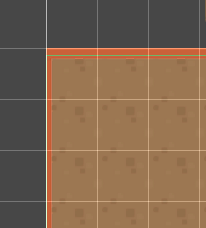
\includegraphics[width=200px]{figuras/tiles.png}
    \caption{Tiles}
    \label{fig_tiles}
\end{figure}
Cada pequeno quadrado é um Tile, e junção de tais Tiles formam algo, como uma plataforma, o chão, um obstáculo. E esta ferramenta auxilia podendo desenhar tais formatos que estes tiles serão arranjados pelo cenário. 
\footnote{Mais informações: \url{https://www.youtube.com/watch?v=ryISV_nH8qw&ab_channel=Brackeys}} 
\footnote{Mais informações: \url{https://github.com/Unity-Technologies/2d-extras}}
\footnote{Mais informações: \url{https://docs.unity3d.com/Manual/Tilemap-Palette.html}}

\subsection{Localization}
Ferramenta auxiliadora para a adição de idiomas no jogo. Por meio de tabelas que representam entidades. Como por exemplo a tabela de itens. \footnote{Mais informações: \url{https://docs.unity3d.com/Packages/com.unity.localization@1.0/manual/index.html}}
\begin{table}[h]
    \centering
    \begin{tabular}{|l|l|l|}
        \hline
          & português        & inglês      \\ \hline
        0 & ferro            & iron        \\ \hline
        1 & ouro             & gold        \\ \hline
    \end{tabular}
\caption{Tabela de exemplo Localzation}
\label{table:localization}
\end{table}
Neste exemplo, durante o desenvolvimento do jogo, em situações onde textos devem ser traduzidos, podemos referenciar os nomes pelo ID da tabela, e o jogo a partir do momento em que está localizado em algum idioma, substitui a referência do texto pela sua versão do idioma selecionado.

\subsection{Animator}
Ferramenta nativas do Unity para inserção de animações nos jogos, por meio desta ferramenta podemos encadear ações para iniciar uma animação específica, como por exemplo: Ao apertar o botão Espaço devemos sair da animação padrão para a animação de pulo. A partir de uma máquina de estados de animações.\footnote{Mais informações: \url{https://docs.unity3d.com/ScriptReference/Animator.htmll}}
\begin{figure}[!h]
    \centering
    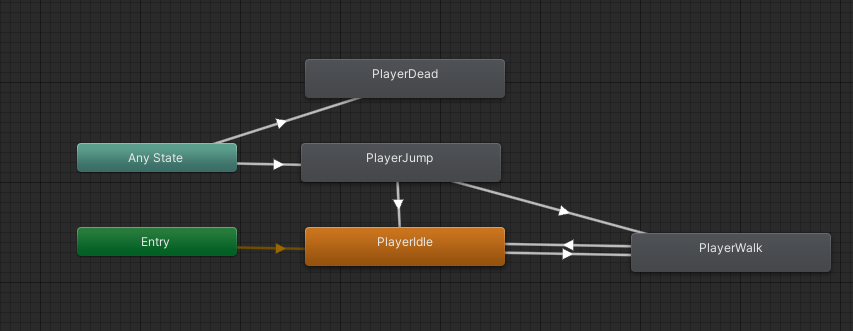
\includegraphics[width=400px]{figuras/animator.png}
    \caption{Exemplo de animator do personagem Weee}
    \label{fig_animator}
\end{figure}
Neste exemplo, a animação padrão é PlayerIdle, e a partir desta animação podemos ir para PlayerWalk. Em PlayerWalk podemos voltar para PlayerIdle ou ir para PlayerJump. Em PlayerJump podemos voltar para PlayerIdle. A partir de qualquer estado podemos ir para PlayerJump ou PlayerDead

\section{Linguagens de Programação}
C\# é uma linguagem de programação orientada a objetos desenvolvida pela Microsoft. Ela é amplamente utilizada em aplicativos de desktop, aplicativos móveis, jogos e sistemas web. C\# possui uma sintaxe semelhante a outras linguagens de programação como C++ e Java, o que a torna fácil de aprender para aqueles já familiarizados com essas linguagens. Além disso, C\# possui uma ampla variedade de recursos e bibliotecas, como suporte ao .NET Framework, que tornam mais fácil para os desenvolvedores criarem aplicativos de alta qualidade e funcionalidade.
\par
C\# é uma linguagem de programação de alto nível, o que significa que ela é mais fácil de ler e escrever do que linguagens de baixo nível como o Assembly. Isso a torna uma opção atraente para aqueles que desejam criar aplicativos complexos sem se preocupar tanto com os detalhes de baixo nível.
\par
C\# também possui um forte suporte à programação paralela, o que permite que os desenvolvedores criem aplicativos que aproveitam ao máximo a potência dos processadores multicore. Além disso, C\# é uma linguagem de programação compilada, o que significa que o código é convertido em um formato de máquina antes de ser executado. Isso pode levar a um desempenho ligeiramente superior em comparação com linguagens interpretadas, como Python.

\section{Formato de Jogo}
O jogo será no formato 2D com mini games que serão jogos digitalizados baseados nos jogos físicos presentes em \cite{bell1998computerIHC}
Neste trabalho, pretende-se auxiliar na absorção do conteúdo da disciplina de forma lúdica. 
% 4) Metodologia (apenas Passo a Passo) (OK)
\chapter{Desenvolvimento}
\label{desenvolvimento}
Desenvolvimento sob a perspectiva da Interação Humano-Computador. "Organização do Espaço de Problema e Análise de Tarefas" que aborda a importância de compreender as características dos usuários e seu relacionamento com a tecnologia. Destaca-se a necessidade de agrupar os usuários por características semelhantes para desenvolver interfaces adequadas às suas necessidades. Em seguida, são apresentadas as subseções: "Perfil de usuário", que descreve as características dos usuários-alvo do projeto; "Personas", que apresenta duas personas específicas com seus objetivos e interesses; "Cenários - Análise de cenário de problema", que descreve a aplicação do jogo What Weee Are em uma sala de aula e a experiência de duas pessoas jogando; e "Análise Hierárquica de Tarefas", que inclui figuras com a análise detalhada das tarefas envolvidas no jogo.

\section{Organização do Espaço de Problema e Análise de Tarefas}
A organização do espaço de trabalho é fundamental para garantir uma interação humano-computador (IHC) eficaz e eficiente. Para isso, é preciso levar em consideração uma série de fatores, como a descrição detalhada das características dos usuários, suas necessidades, habilidades e limitações, sua relação com a tecnologia e o ambiente em que irão utilizar o sistema. No contexto da IHC, é importante compreender o perfil dos usuários que irão interagir com o sistema, incluindo informações como idade, nível de escolaridade, habilidades técnicas, experiência com tecnologia e com o tema específico do sistema em questão. Essas informações podem ser obtidas por meio de pesquisas de campo, entrevistas e estudos de usabilidade. Ao agrupar os usuários por características semelhantes, é possível ambientar melhor o projeto, com interfaces e funcionalidades que atendam às necessidades específicas de cada grupo de usuários. Por exemplo, no presente trabalho, o foco está em pessoas de idade escolar, com interesse em tecnologia e baixa experiência ou contato com assuntos ambientais. Nesse caso, a organização do espaço de trabalho deve levar em consideração essas características e desenvolver interfaces intuitivas e amigáveis, com informações e funcionalidades relevantes para esse público específico.

Alessio desempenhou um papel central na co-criação do projeto What Weee Are, atuando como principal idealizador e contribuindo significativamente para a concepção e desenvolvimento do jogo. As interações iniciais ocorreram por meio de duas reuniões realizadas via Google Meet, nas quais Alessio compartilhou suas ideias iniciais e contribuiu para a elaboração da estrutura do jogo, incluindo a ideia de desmontar itens durante o jogo, a obtenção de poderes e a criação de quatro fases distintas.

Além disso, Alessio contribuiu fornecendo arte para ser utilizada no jogo e participou ativamente das decisões relacionadas às fases, que foram definidas como cozinha, jardim, metrô e vulcão. Sua origem italiana foi fundamental para a tradução do jogo para o idioma, e ele também ofereceu sugestões valiosas para a implementação de detalhes importantes no jogo. Como resultado de sua colaboração, o jogo What Weee Are se tornou um produto mais completo e diversificado, com uma abrangência maior e a possibilidade de atender a um público internacional.

\subsection{Perfil de usuário}
Sob a óptica de IHC, se trata da descrição detalhada das características dos usuários, sua relação com tecnologia, seu conhecimento sobre domínio e tarefas, agrupar usuários por características semelhantes. Neste trabalho, o foco são em pessoas de idade escolar majoritariamente, mas não excludente à pessoas fora desta faixa. Com interesse por tecnologias e com baixa experiência ou contato pelo assunto ambiental. Olhar tabela \ref{table:personasTable}
\begin{table}[h]
    \centering
    \begin{tabular}{|l|l|l|}
        \hline
                                 & Aluno A     & Aluno B      \\ \hline
        Faixa etária             & 5 a 12 anos & 13 a 17 anos \\ \hline
        Interesse por tecnologia & sim         & sim          \\ \hline
        Experiência ambiental    & baixa       & baixa        \\ \hline
    \end{tabular}
\caption{Tabela de personas}
\label{table:personasTable}
\end{table}

\subsection{Personas}
João Pedro é um professor da Escola Estadual João Carlos Gomes Cardim, em Diadema, hoje leciona para o quinto ano do ensino fundamental. Gosta de trazer aulas dinâmicas aos alunos, pois entende que isso os prende com maior atenção ao que está sendo lecionado. Entende que o uso da tecnologia no ensino pode ser uma ferramenta muito auxiliadora, uma vez que, os alunos gostam de ficar conectados e praticamente passaram a vida toda em contato com o mundo digital.
Têm como objetivos pessoais promover uma educação ativa com os alunos, colocar em evidência os Objetivos de Desenvolvimento Sustentável para os alunos.
Objetivos Pessoais: 
- Aprimorar o aprendizado de seus alunos sobre os problemas causados pelo desperdício de materiais eletrônicos.

Objetivos Práticos:
- Levar um jogo divertido sobre o assunto aos seus alunos;
- Engajar os alunos sobre assuntos que normalmente são ignorados.


Natália é aluna do sexto ano do ensino fundamental e aluna do professor João Pedro. Gosta de videogames, assim como outras crianças de sua idade, possui um interesse grande em tecnologia e pelo mundo digital.

Leonardo é aluno do primeiro ano do ensino médio, da Escola Estadual João Carlos Gomes Cardim, em Diadema. Possui interesse em cursar faculdade de biologia na UFABC, pois após uma visita a instituição chegou a informação da interdisciplinaridade e vê isso como uma boa oportunidade de realizar projetos envolvendo biologia e computação, que é o seu segundo interesse.

\subsection{Cenários - Análise de cenário de problema}
\label{cenarios}
O Professor João Pedro, resolveu trazer novas maneiras de ministrar suas aulas sobre sustentabilidade, e viu uma oportunidade de fazer isso via jogos digitais, uma vez que tem conhecimento da preferência de seus alunos por tecnologia. Trouxe para a turma do sexto ano, de Natália, o jogo digital What Weee Are para abordar tais assuntos de maneira lúdica e mais ativa por partes dos alunos, uma vez que eles que irão interagir com o sistema. A ideia é requisitar uma redação sobre reciclagem de materiais eletrônicos antes e após a partida jogada pelos alunos. O Professor acredita que a apresentação do jogo aos alunos irá proporcionar dinamismo e maior interesse dos alunos ao assunto sobre desperdício de materiais eletrônicos.

Natália iniciou o jogo lendo um breve diálogo explicando quais são os problemas ali enfrentados e de quais maneiras poderá ajudar a resolver este empasse. Utilizando as teclas A e D do teclado para se movimentar (A para esquerda, D para direita), ESPAÇO para pular e J para interagir com objetos e avanço de diálogos. Inicialmente houveram dificuldades para progredir, pois não foram coletados os materiais mal descartados no jogo, que são usados para possibilitar a progressão, ao entender que era necessário a coleta dos itens a dificuldade deixou de ser um problema. Natália ficou muito animada ao perceber que seu personagem poderia ficar mais forte ao progredir no jogo.

Leonardo iniciou o jogo muito interessado pelo sistema de construção e desconstrução, imaginando muitas possibilidades de novos itens e maneiras que o personagem pudesse ficar mais fortes, tentando diversas combinações de materiais para criação de outro que seja útil para progressão, logo de cara entendeu que a coleta dos recursos pelos mapas do jogo seria crucial para a evolução do jogo. Sentiu que o jogo poderia apresentar uma maior dificuldade para que houvesse mais desafios e que houvessem novas fases no jogo.

\subsection{Análise Hierárquica de Tarefas}
\begin{figure}[h]
    \centering
    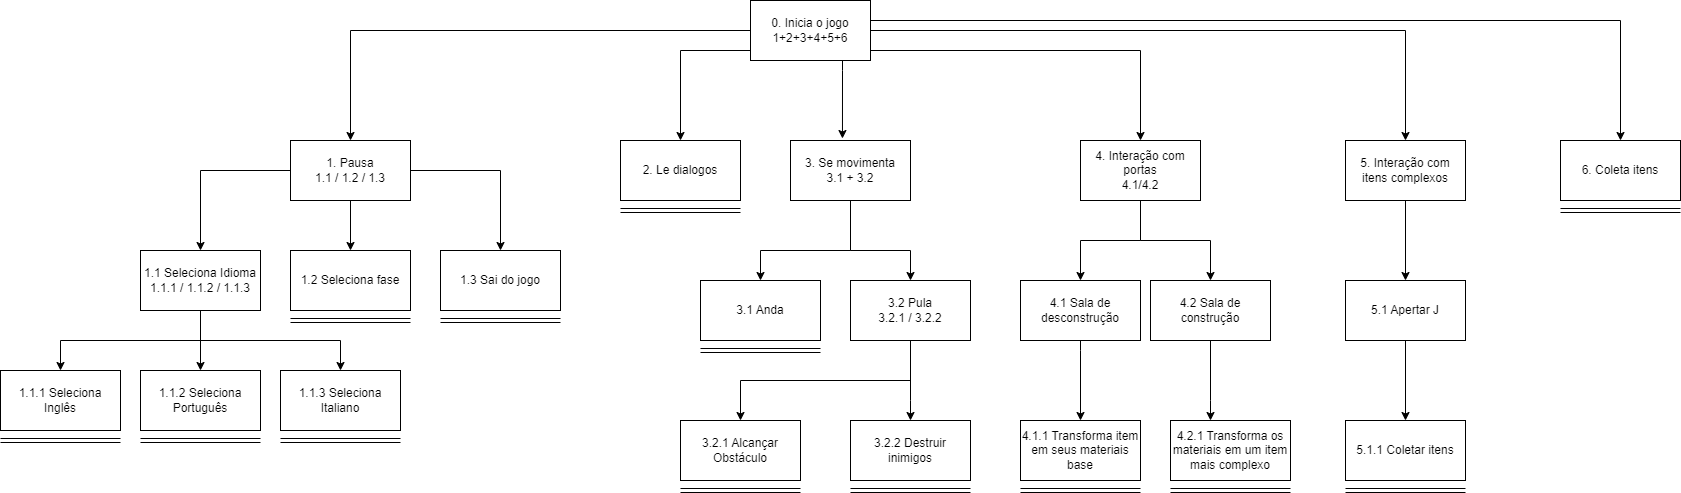
\includegraphics[width=\textwidth]{figuras/analise_tarefas.drawio.png}
    \caption{Análise Hierárquica de Tarefas}
    \label{fig_analise_hierarquica}
\end{figure}

\begin{figure}[h]
    \centering
    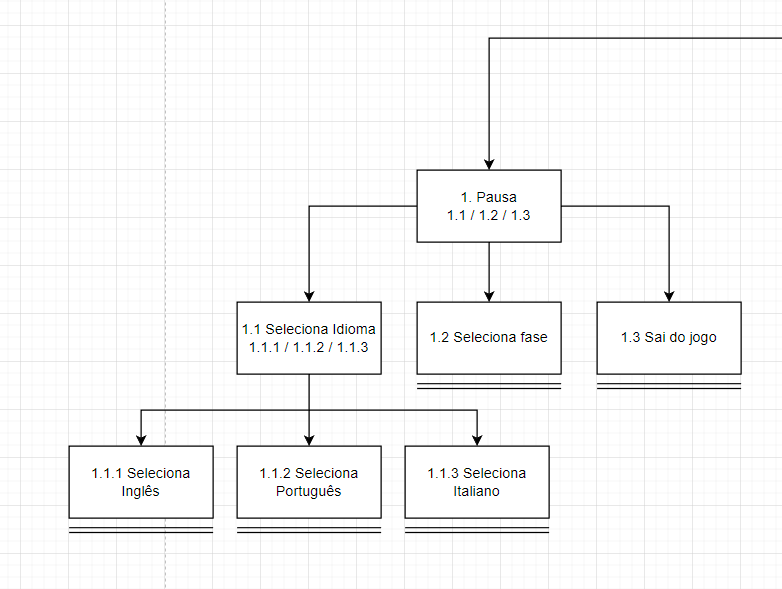
\includegraphics[width=\textwidth]{figuras/aht-a.png}
    \caption{Análise Hierárquica de Tarefas - A}
    \label{fig_analise_hierarquica_a}
\end{figure}
\begin{figure}[h]
    \centering
    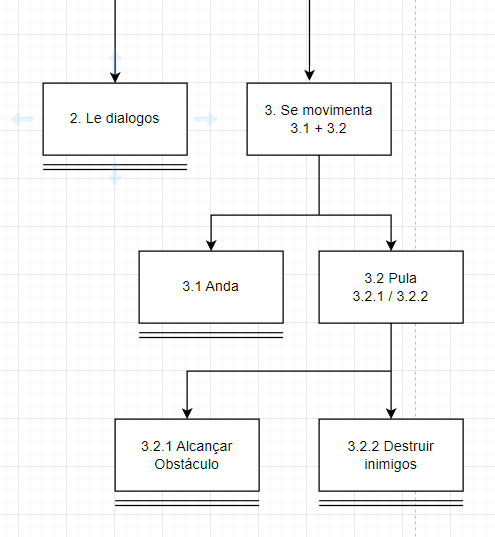
\includegraphics[width=\textwidth]{figuras/aht-b.png}
    \caption{Análise Hierárquica de Tarefas - B}
    \label{fig_analise_hierarquica_b}
\end{figure}
\begin{figure}[h]
    \centering
    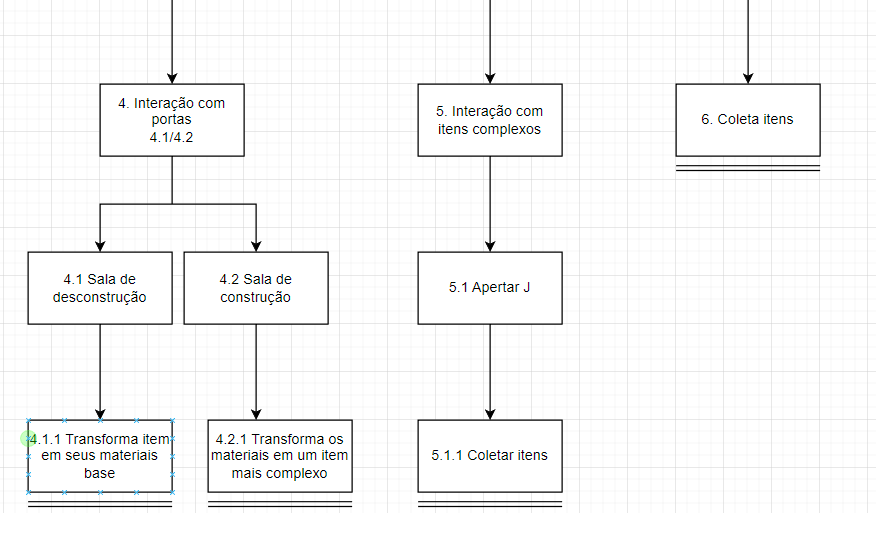
\includegraphics[width=\textwidth]{figuras/aht-c.png}
    \caption{Análise Hierárquica de Tarefas - C}
    \label{fig_analise_hierarquica_c}
\end{figure}

\chapter{Desenvolvimento Técnico}
Neste capítulo será abordada as técnicas e escolhas de desenvolvimento aplicadas durante o projeto para que o jogo fosse finalizados. Como são os scripts, padrões de projetos e algumas mecânicas e interações presentes em What Weee Are.

\label{desenvolvimento_tecnico}
\section{Scripts}
No moto gráfico Unity, os comportamentos e aspectos ligados às mecânicas do jogo são implementadas via scripts, scripts na linguagem de programação C\#. Scripts atrelados a algum elemento do jogo, devem herdar uma classe chamada MonoBehaviour \footnote{Mais informações \url{https://docs.unity3d.com/ScriptReference/MonoBehaviour.html}} que implementa e nos dá interfaces para adicionar os comportamentos particulares dos elementos do jogo.
Tais scripts são utilizados para implementar aspectos como: movimentação do personagens e inimigos, coleta de itens, emitir eventos após algum acontecimento. Importante atentar a possibilidade de uso de Design Patterns para organizar e mitigar repetições de códigos, alguns padrões de projeto utilizados foram Singleton e Observer.
\subsection{Singleton}
Singleton é uma classe que possui apenas uma instância, possibilitando acesso e controle global. Utilizada para implementar o GameManager, uma classe onde é necessário haver apenas uma única instância, pois é nesta classe que controlamos qual estágio estamos, quais itens coletados, quantas vidas possuí, tempo de jogo. Informações que não pode correr o risco de ter dois ou mais valores.

\subsection{Observer}
Padrão de projeto muito interessante, onde outros objetos observam e aguardam mudanças de outro objeto. Muito importante para implementar casos onde por exemplo, no desmontador de itens, queremos que a cada item depositado nas caixas, queremos testar se algum item mais complexo pode ser gerado. Ou seja, na mudança de estado da caixa de entrada, notificamos o testador de criação. Este padrão nos ajuda a emitir vários eventos à cada mudança, para quem deseja saber das mudanças, tirando a responsabilidade do emissor de saber quem o está observando, a responsabilidade é do objeto interessado de se inscrever para saber das mudanças.

\section{Gerenciador de Diálogos}
No Gerenciador de Diálogos, uma única classe capaz de apresentar os diálogos, imprimindo os parágrafos lentamente e permitindo ir para o próximo parágrafo. Necessitando receber apenas um objeto da classe Dialogue, que contém as frases a serem apresentadas em uma lista, enfileirando todas as sentenças(cada item da lista) do diálogo e imprimindo caractere por caractere, ao finalizar a sentença, inicia a próxima.
\subsection{Dialogo}
Classe Dialogue, implementada para ser capaz de localizar os textos em cada um dos três idiomas(inglês, português e italiano), a quantidade de sentença, as sentenças e quem está apresentando este diálogo.

\break
\section{Inventário}
Implementado para ser capaz de inserir novos itens, adicionar existentes e remove-los quando necessário. Além de a cada operação, os dados são persistidos em formato de arquivo JSON \footnote{Mais informações: \url{https://www.json.org/json-pt.html}} para que o progresso de coleta de itens não seja perdido caso a Unity decida recriar o objeto de Inventário, ou caso o jogo seja finalizado e após um tempo retomado. 
\par
Faz uso de outra estrutura chamada ItemDatabase, sendo responsável por carregar as informações de todos os itens do jogo definidas num arquivo JSON e leva-las ao jogo. Foi uma forma de facilitar a inserção de novos itens ao jogo, sendo necessário apenas adicionar um novo objeto JSON ao arquivo de definição com as informações necessárias para adicionar o item. Possuindo algumas informações necessárias, como identificador único, nome (importante que a imagem do item possua o mesmo nome do item, e esteja localizada em: \url{./Assets/StreamingAssets/Sprites/items/ingame_sprites/}), a descrição, se é isRaw(item primitivo, que não pode ser desmontado), caso falso, necessita a definição de uma lista rawItems, no qual é necessário apontar o identificador do item em que se transforma, e na quantidade. Ver \ref{fig_item_json_definition}.
\begin{figure}[h]
    \centering
    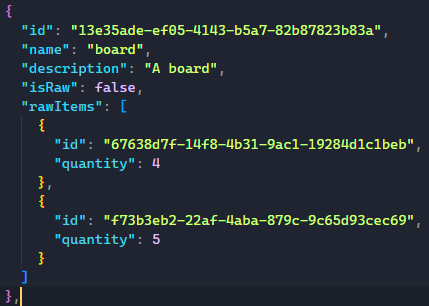
\includegraphics[width=300px]{figuras/item_definition.png}
    \caption{Definição de itens}
    \label{fig_item_json_definition}
\end{figure}


\section{Inimigos}
Os inimigos precisam ser desafiadores e não caírem das plataformas quando chegam em suas bordas, para isso foi implementado um Script chamado AIPatrol, uma inteligência artificial bem simplificada que faz com que os inimigos patrulhem uma área e voltem caso cheguem no fim da plataforma. Fazendo uso de um BoxCollider2D \footnote{https://docs.unity3d.com/Manual/class-BoxCollider2D.html}. Usando um componente adicional que checa se um circulo não visível, que fica a frente do inimigo, deixa de encostar na plataforma.
\begin{figure}[h]
    \centering
    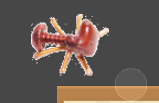
\includegraphics[width=300px]{figuras/GroundChecker.png}
    \caption{Exemplo do Checador de Chão, usado na IA dos inimigos}
    \label{fig_ground_checker}
\end{figure}


% 5) Cronograma (OK)
%\include{secoes/cronograma}
% -----------------------------
% 6) Análise e modelagem do sistema: Análise de Requisitos (pendente), Casos de Uso (OK) , fluxograma de telas (OK - tirar do anexo).
%-----------------------------
% 7)  Implementação do Sistema: Telas presentes no sistema, associando cada uma delas a cada um dos casos de uso.
\chapter{Resultados: What Weee Are Game}
\label{resultados}

Neste capítulo é detalhado aspectos presentes do jogo "What Weee Are" e os motivos da escolha. A história se desenrola em quatro cenários: Cozinha, Jardim, Metrô e Vulcão, descrição das personagens, explicação da escolha dos planos de fundo e o enredo do jogo estão presentes neste capítulo. Todos os detalhes de implementação, aplicabilidade e escolhas para o jogo, as explicações de mecânicas como o sistema de crafting e a discussão final.

\section{Enredo}
Em "What Weee Are", somos apresentados a Weee, o herói da história que enfrentará desafios e se fortalecerá para combater a Eco-InterCrim, a grande vilã da aventura. Weee tem como objetivo coletar os materiais descartados incorretamente ao longo de sua jornada e usá-los para limpar o planeta das mãos da Eco-InterCrim, organização criminosa responsável pela poluição do meio ambiente por meio do descarte inadequado de resíduos eletrônicos.

Acompanhando Weee em sua missão, está o Grilo Falante, um sábio guia que fornece informações sobre a situação e orienta o personagem jogável pelo mundo, explicando o que deve ser feito para progredir. O Grilo Falante aparece em diálogos ao longo do jogo e no início de cada cenário, fornecendo instruções e contexto para a jornada de Weee.

A aventura se inicia no cenário da Cozinha, onde o Grilo Falante revela os problemas causados pelo descarte inadequado de resíduos eletrônicos e apresenta a Eco-InterCrim como a possível responsável por essa situação. Weee deve enfrentar desafios como coletar itens e derrotar formigas vermelhas e verdes, culminando em um confronto com a Aranha Mecânica, o desafio final do cenário.

No cenário do Jardim, Weee recebe a informação de que pode adquirir uma nova habilidade, o pulo-duplo, para investigar possíveis contaminações. O Grilo Falante indica a necessidade de voltar à Cozinha para coletar mais itens e construir essa nova habilidade. Ao chegar no Jardim, Weee encontra fluidos poluentes, agravando a situação e indicando a gravidade dos crimes ecológicos cometidos pela Eco-InterCrim.

O próximo cenário é o Metrô, onde o Grilo Falante revela que a Eco-InterCrim está usando a malha ferroviária para disseminar seus crimes ambientais por meio do plano chamado Toxicity. Weee deve avançar até o vulcão, enfrentando desafios e coletando itens, como o potencializador de pulos, para aprimorar suas habilidades e combater a organização.

O último desafio ocorre no cenário do Vulcão, onde a base da Eco-InterCrim está localizada. Weee enfrenta riscos, como a presença de lava, enquanto busca acabar com os planos da organização criminosa. Ao finalizar essa etapa, Weee é parabenizado por seu feito heroico e é informado de que agora é necessário lidar com os danos causados pela Eco-InterCrim.

O jogo termina com a missão de Weee retornar à Cozinha para coletar mais itens e auxiliar na reconstrução do planeta. Embora haja o risco de que a Eco-InterCrim volte a atacar, Weee está agora ciente da identidade dos responsáveis e está determinado a impedir que os crimes ecológicos ocorram novamente, protegendo o meio ambiente.

%\section{What Weee Are: The Game}
\section{Personagens}
A escolha de todos os personagens e inimigos é resultado de uma colaboração criativa liderada por Alessio, que já vinha desenvolvendo criaturas feitas exclusivamente a partir de materiais eletrônicos reciclados. Sua participação artística foi fundamental ao fornecer as ilustrações que compõem o jogo. A inclusão de personagens construídos a partir de materiais reciclados serve como uma poderosa forma de reforçar a mensagem central do jogo em relação ao tema ambiental.

What Weee Are possui dois personagens principais. Weee, a formiga e o Grilo Falante. Weee é nosso personagem controlável, onde iremos andar e explorar pelos quatro cenários que encontramos no jogo, Weee será capaz de coletar itens, destruir itens complexos, montar itens, desmontar itens, adquirir novas habilidades, derrotar inimigos e assim progredir cada vez mais pelo mundo.

Weee é o herói da história, que irá enfrentar os desafios, se fortalecer e por fim enfrentar o grande inimigo da aventura, a Eco-InterCrim. Weee coletará os materiais descartados incorretamente e propositalmente ao longo da jornada, usará tudo que tiver disponível para alcançar o seu objetivo de limpar o planeta das mãos da Eco-InterCrim

\begin{figure}[h]
    \centering
    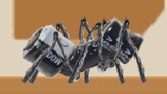
\includegraphics[width=150px]{figuras/weee.png}
    \caption{Weee - o personagem jogável}
    \label{fig_weee}
\end{figure}
\par
O Grilo Falante é o guia de Weee, é quem irá contar o que está acontecendo e direcionará o personagem jogável pelo mundo e o que deverá fazer para progredir. Haverão diálogos durante o jogo e no início dos cenários onde o Grilo irá aparecer para interagir.
\begin{figure}[h]
    \centering
    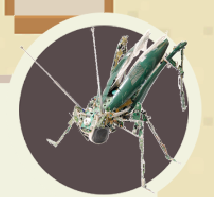
\includegraphics[width=150px]{figuras/grilo.png}
    \caption{Grilo Falante - o guia}
    \label{fig_grilo}
\end{figure}

\section{Cenários}
Esta seção apresentará quatro cenários distintos do jogo "What Weee Are": Cozinha, Jardim, Metrô e Vulcão. A escolha desses planos de fundo tem como objetivo demonstrar aos jogadores as consequências resultantes do descarte inadequado de materiais eletrônicos. Cada cenário representa uma situação única em que problemas relacionados ao descarte incorreto podem afetar tanto o ambiente doméstico quanto a sociedade em geral. Através dessas experiências virtuais, os jogadores serão confrontados com desafios que vão desde questões pessoais, como problemas dentro de casa, até problemas sociais, como a tentativa de contaminação do solo. O objetivo é fornecer uma perspectiva abrangente sobre os impactos negativos que a falta de gerenciamento adequado dos resíduos eletrônicos pode causar em diferentes contextos, incentivando assim a conscientização e a adoção de práticas sustentáveis.

\subsection{Fase 1 - A Cozinha}
Descrição: Nesta fase do jogo, somos apresentados ao que iremos enfrentar e algumas noções básicas do jogo. Aqui o Grilo Falante diz sobre como faremos a movimentação e como progredir durante a primeira fase. Irá dizer o que está acontecendo sobre o desperdício de materiais eletrônicos e quem possivelmente está causando isso. Devido ao abandono dos materiais em locais inapropriados, começaram a vazar substâncias tóxicas para o meio ambiente, e introduzirá a organização Eco-InterCrim como possíveis responsáveis pelo desastre.
Aparecerão alguns itens a serem coletados e algumas formigas vermelhas e verdes para enfrentar, além de uma Aranha Mecânica no final que será o maior desafio presente.

Sua escolha vêm como forma de apresentar o problema do descare incorreto dos materiais eletrônicos, mostrando que o problema também pode afetar em nossos ambientes privados. Além também de ser um estágio introdutório, pois o jogo segue uma linha de progressão entre os cenários.
\begin{figure}[h]
    \centering
    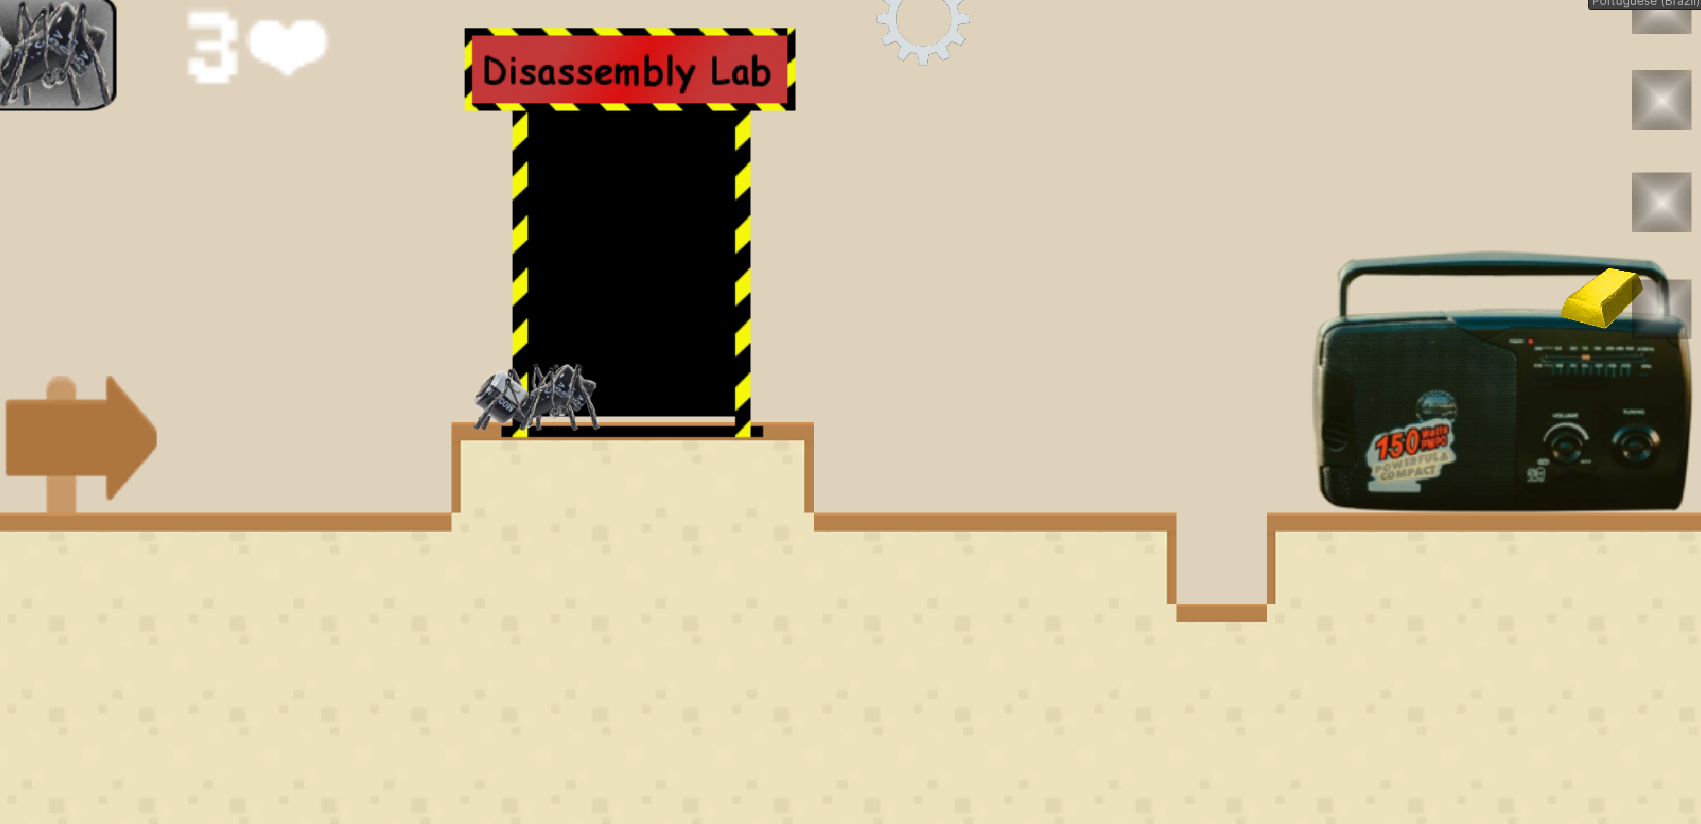
\includegraphics[width=300px]{figuras/cozinha.png}
    \caption{Fase 1 - A cozinha}
    \label{fig_cozinha}
\end{figure}

Música utilizada "Cookie Island" \cite{CookieIsland}

\subsection{Fase 2 - Jardim}

Descrição: Nesta etapa, o Grilo Falante nos dirá que é possível conseguir uma nova habilidade, o pulo-duplo e com isso investigar possíveis contaminações no Jardim. É informado da possibilidade de voltar à cozinha para coletar mais itens para ajudar a construir a nova habilidade.

A escolha do jardim vem como uma proposta de transição o lado de dentro (casa) e o mundo exterior, um estágio para servir como uma transicão entre a cozinha e o metrô.
\begin{figure}[h]
    \centering
    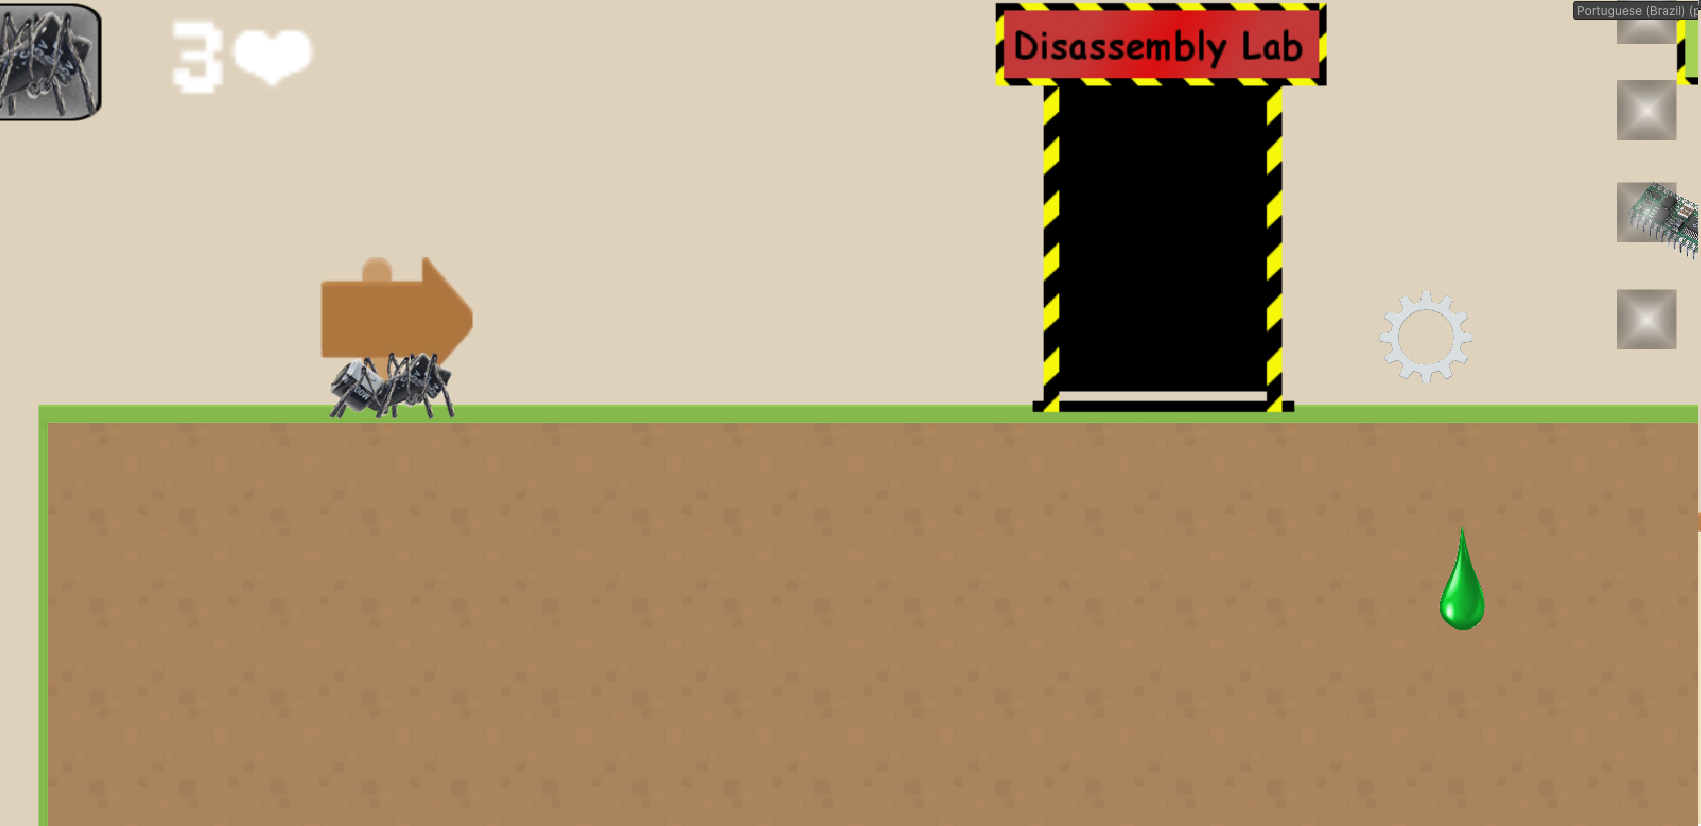
\includegraphics[width=300px]{figuras/jardim.png}
    \caption{Fase 2 - O jardim}
    \label{fig_jardim}
\end{figure}

Música utilizada "Candy Valley" \cite{CandyValley}

\subsection{Fase 3 - Metrô}
Descrição: Chegando no metrô, o Grilo Falante informa que a Eco-InterCrim está utilizando a malha ferroviária para disseminar seus crimes ambientais com seu plano Toxicity, tomando inicialmente o controle do subsolo e contaminando-o com, aumentando o risco de contaminação dos lençóis freáticos, os objetivos da organização é contaminar o planeta com lixo eletrônico, para que a população fique doente e dependente de seus produtos e serviços, que serão oferecidos como solução para os problemas causados por eles mesmos, a missão passa a ser de coletar o máximo de resíduos(itens) possíveis. 

Este cenário vem como plano de fundo para apresentar problemas sérios que o descarte inadequado pode causar à sociedade, como exemplificado no jogo o problema da contaminação do solo.
\begin{figure}[h]
    \centering
    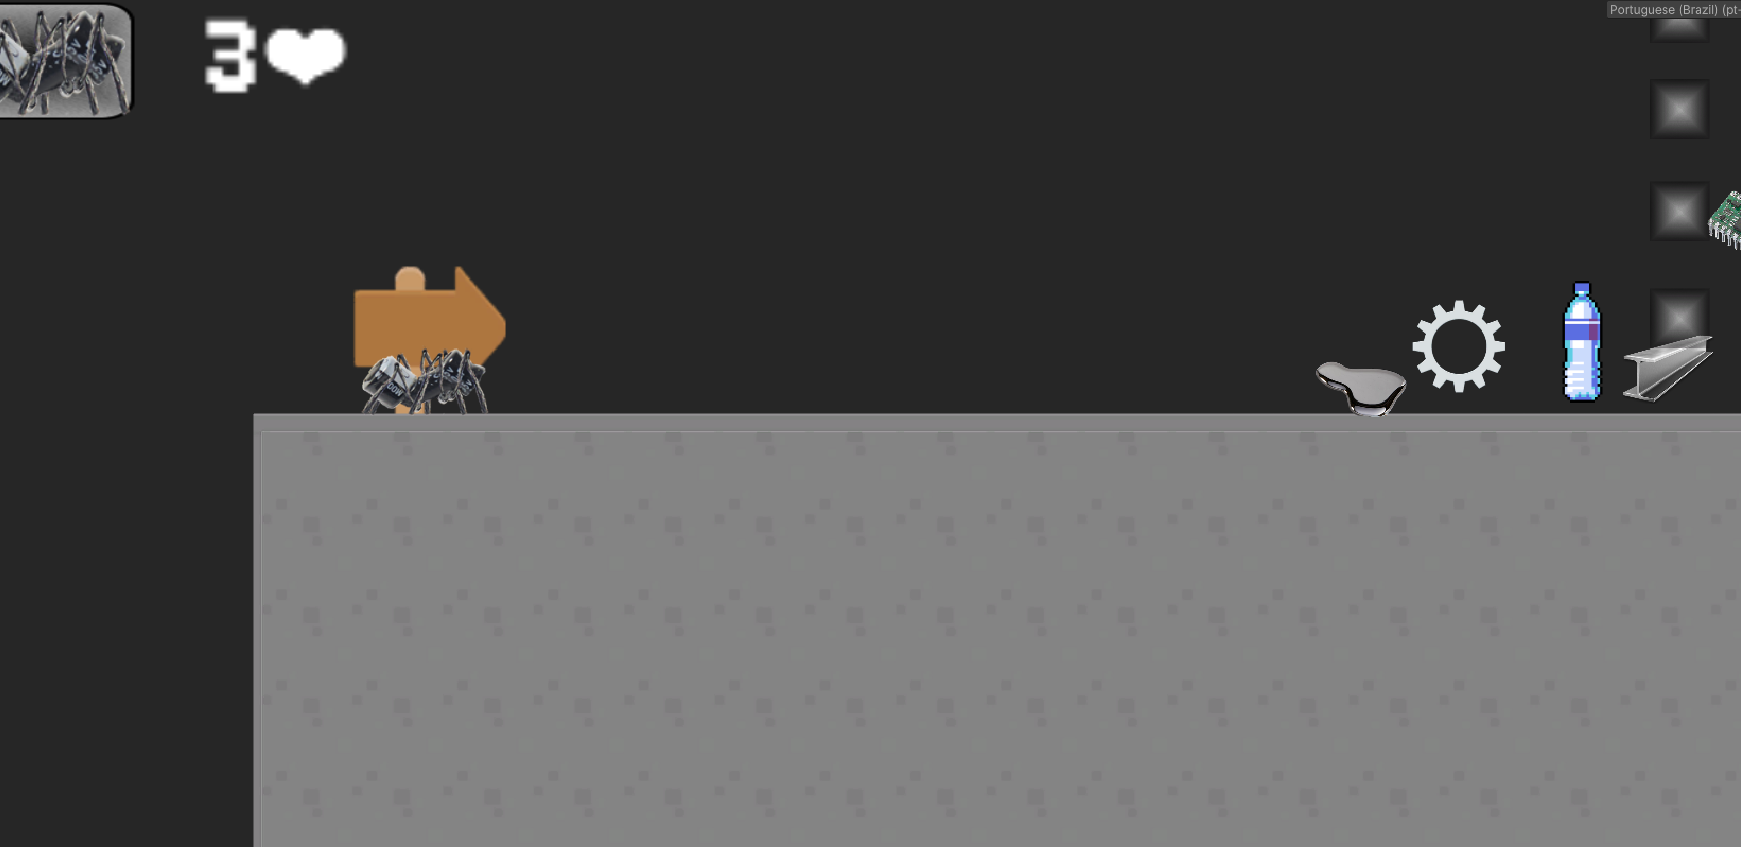
\includegraphics[width=300px]{figuras/metro.png}
    \caption{Fase 3 - O Metrô}
    \label{fig_metro}
\end{figure}

Música utilizada "Cyber Soldier" \cite{CyberSoldier}
\pagebreak

\subsection{Fase 4 - Vulcão}
O último desafio é o vulcão, aqui que está a base da Eco-InterCrim, onde finalmente será possível impedir que as investidas contra o meio ambiente tenham sucesso. Ao finalizar, Weee é parabenizada pelo seu feito heroico e que agora devemos cuidar dos danos causados pela organização criminosa.

Por fim este cenário foi escolhido como uma maneira de apresentar algo grandioso, um cenário de maior impacto visual e que passe a sensação de que algo importante está acontecendo no momento, justamente por ser o último estágio.
\begin{figure}[hbt!]
    \centering
    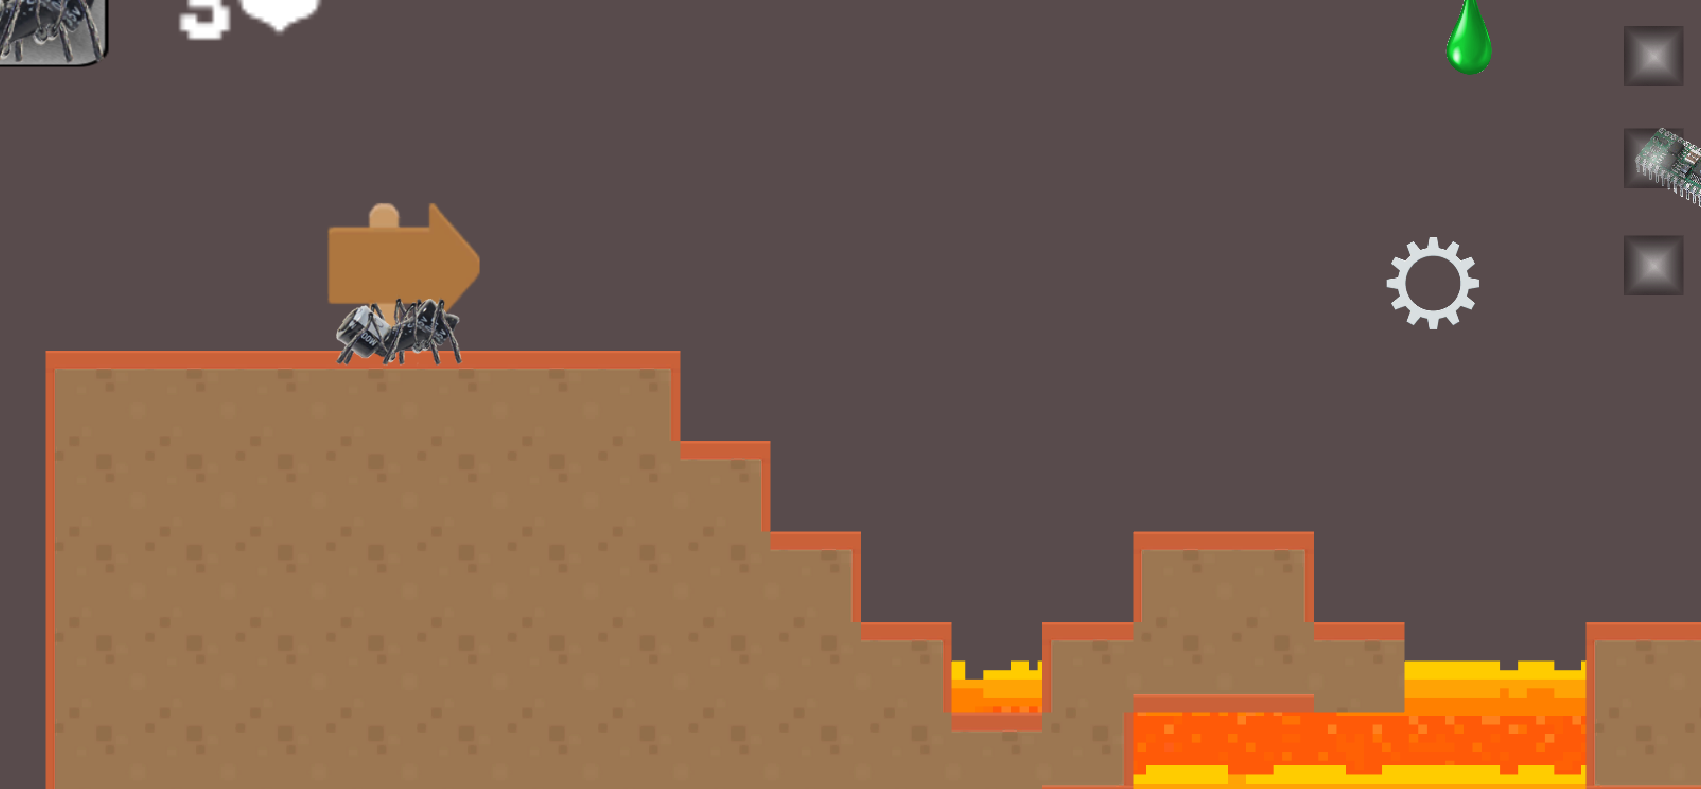
\includegraphics[width=300px]{figuras/vulcao.png}
    \caption{Fase 4 - O Vulcão}
    \label{fig_vulcao}
\end{figure}

Música utilizada "Final Act" \cite{FinalAct}

\section{Itens}
A seguir estão todos os itens presentes no jogo e a receita para construí-los (se possível), a existência também de alguns itens do jogo que podem aplicar algum efeito em Weee (e.g A bateria). As escolhas dos itens são justamente por serem subprodutos e resíduos eletrônicos e assim manter o tema central abordado no jogo e justificarem o uso do Sistema de \textit{Crafting} \ref{craft}
\label{list:itens}
\begin{itemize}
    \item Placa - Pode ser desmontado em ouro e ferro
    \item Cobre
    \item Engrenagem - Pode ser desmontado em prata
    \item Ouro
    \item Bateria - Dá vida à Weee, pode ser criado a partir de Aço e Mercúrio
    \item Ferro
    \item Mercúrio
    \item Plástico
    \item Prata
    \item Aço - Pode ser produzido a partir de 6 unidades de Ferro
\end{itemize}

\pagebreak
\section{Melhorias}
As melhorias a seguir, propõem a possibilidade da reciclagem dos materiais coletados durante as partidas pelos jogadores. Estas melhorias foram escolhidas como forma de trazer a sensação de progresso aos jogadores, confeccionadas por meio da reciclagem dos materiais coletados durante as fases do game.
\begin{itemize}
    \item Ganho de velocidade - Aumenta a velocidade por tempo determinado - Pode ser criado a partir de 14 únidades de placa e 10 unidades de engrenagem;
    \begin{figure}[hbt!]
        \centering
        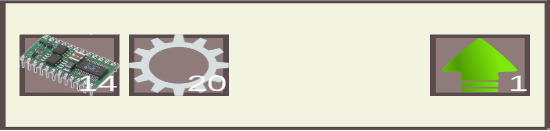
\includegraphics[width=300px]{figuras/receita_double_speed.png}
        \caption{Ganho de velocidade}
        \label{fig_receita_double_speed}
    \end{figure}
    
    \item Bateria - Dá vida à Weee - Pode ser criado a partir de Aço e Mercúrio;
    \begin{figure}[hbt!]
        \centering
        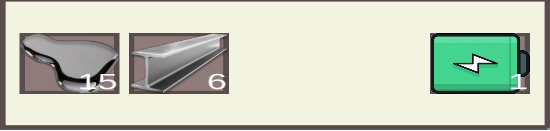
\includegraphics[width=300px]{figuras/receita_vida.png}
        \caption{Bateria}
        \label{fig_receita_vida}
    \end{figure}
    
    \item Pulo Duplo - Permite Weee realizar dois pulos subsequentes - Pode ser criado a partir de 12 unidades de placa, 11 unidades de engrenagem e 7 unidades de ferro;
    \begin{figure}[hbt!]
        \centering
        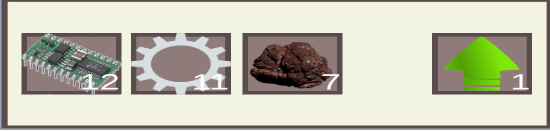
\includegraphics[width=300px]{figuras/receita_double_jump.png}
        \caption{Pulo Duplo}
        \label{fig_receita_double_jump}
    \end{figure}
    
    \item Aumento de Poder - Da a Weee a 4 vezes sua força atual, ideal para derrotar inímigos com um único golpe - Pode ser criado a partir de 14 unidades de mercúrio;
    \begin{figure}[hbt!]
        \centering
        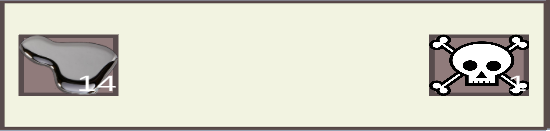
\includegraphics[width=300px]{figuras/receita.png}
        \caption{Aumento de Poder}
        \label{fig_receita_double_damage}
    \end{figure}
    
    \item Aumento de força de pulo - Da a Weee a capacidade de pular mais alto a cada pulo - Pode ser criado a partir de 12 unidades de engrenagem e 14 unidades de plástico.
    \begin{figure}[hbt!]
        \centering
        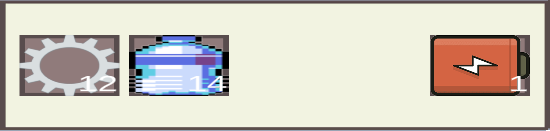
\includegraphics[width=300px]{figuras/receita_jump_force.png}
        \caption{Aumento de força de pul}
        \label{fig_receita_jump_force}
    \end{figure}
\end{itemize}

\section{Inimigos}
Os inimigos estão presentes para adicionar uma certa dificuldade no jogo e deixar a experiência mais divertida.
\begin{description}
    \item[Formigas Vermelhas] Apenas patrulham uma região. Criação artística do Alessio, a escolha deste inimigo vem de manter a estética de personagens insetos eletrônicos. 
    \begin{figure}[h]
        \centering
        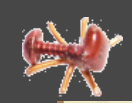
\includegraphics[width=100px]{figuras/redant.png}
        \caption{A Formiga Vermelha}
        \label{fig_redant}
    \end{figure}

    \item[Formigas Verdes] Patrulham uma região e podem pular. Criação artística do Alessio, a escolha deste inimigo vem de manter a estética de personagens insetos eletrônicos. Além de acrescentar uma dificuldade um pouco mais do que as formigas vermelhas.
    \begin{figure}[h]
        \centering
        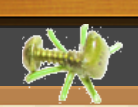
\includegraphics[width=100px]{figuras/greenant.png}
        \caption{A Formiga Verde}
        \label{fig_greenant}
    \end{figure}
    
    \item[Aranhas mecânicas] Possuem alta velocidade e podem pular. Criação artística do Alessio, a escolha deste inimigo vem de manter a estética de personagens insetos eletrônicos. Acrescentam uma dificuldade maior ainda do que das formigas verdes.
    \begin{figure}[h]
        \centering
        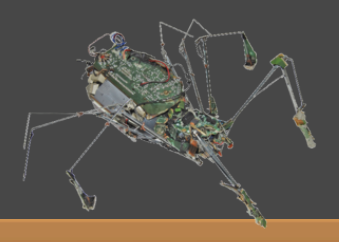
\includegraphics[width=100px]{figuras/spider.png}
        \caption{A Aranha Mecânica}
        \label{fig_spider}
    \end{figure}
\end{description}

\pagebreak
\section{Sistema de Crafting}
\label{craft}
A mecânica de \textit{"crafting"} é um conceito amplamente utilizado no design de jogos eletrônicos, que envolve a criação e destruição de elementos dentro do jogo, proporcionando uma experiência interativa aos usuários e estimulando sua criatividade. A criação e destruição são ações frequentemente presentes nesses jogos, fundamentais para essa mecânica.

Os sistemas de criação presentes nos jogos eletrônicos oferecem uma poderosa ferramenta para a criação de narrativas interativas, envolvendo os jogadores e permitindo a exploração de temas complexos. Para exemplificar esse argumento, o autor concentra-se no jogo de simulação urbana SimCity e em seu sistema de criação, que possibilita aos jogadores projetar e gerenciar cidades. De acordo com \cite{craftingGames}, o uso estratégico desse sistema de criação permite a criação de histórias complexas e interativas, que não apenas proporcionam uma experiência de jogo satisfatória, mas também exploram questões importantes, como o meio ambiente, a justiça social e as políticas públicas.

O sistema de "crafting" incorpora o conceito de reciclagem, permitindo que os jogadores utilizem materiais encontrados durante o jogo. Por meio desse sistema, é possível criar melhorias para o personagem, tornando-o mais forte, além de criar novos itens colecionáveis para a aventura. Dessa forma, esse sistema atribui importância à tarefa de coletar os itens necessários. \ref{list:itens}.

\subsection{Laboratório de desmontagem}
Aplicado os conceitos de Crafting voltados para desmontar itens complexos em itens primitivos, para assim criarmos outras opções de crafting
\begin{figure}[h]
    \centering
    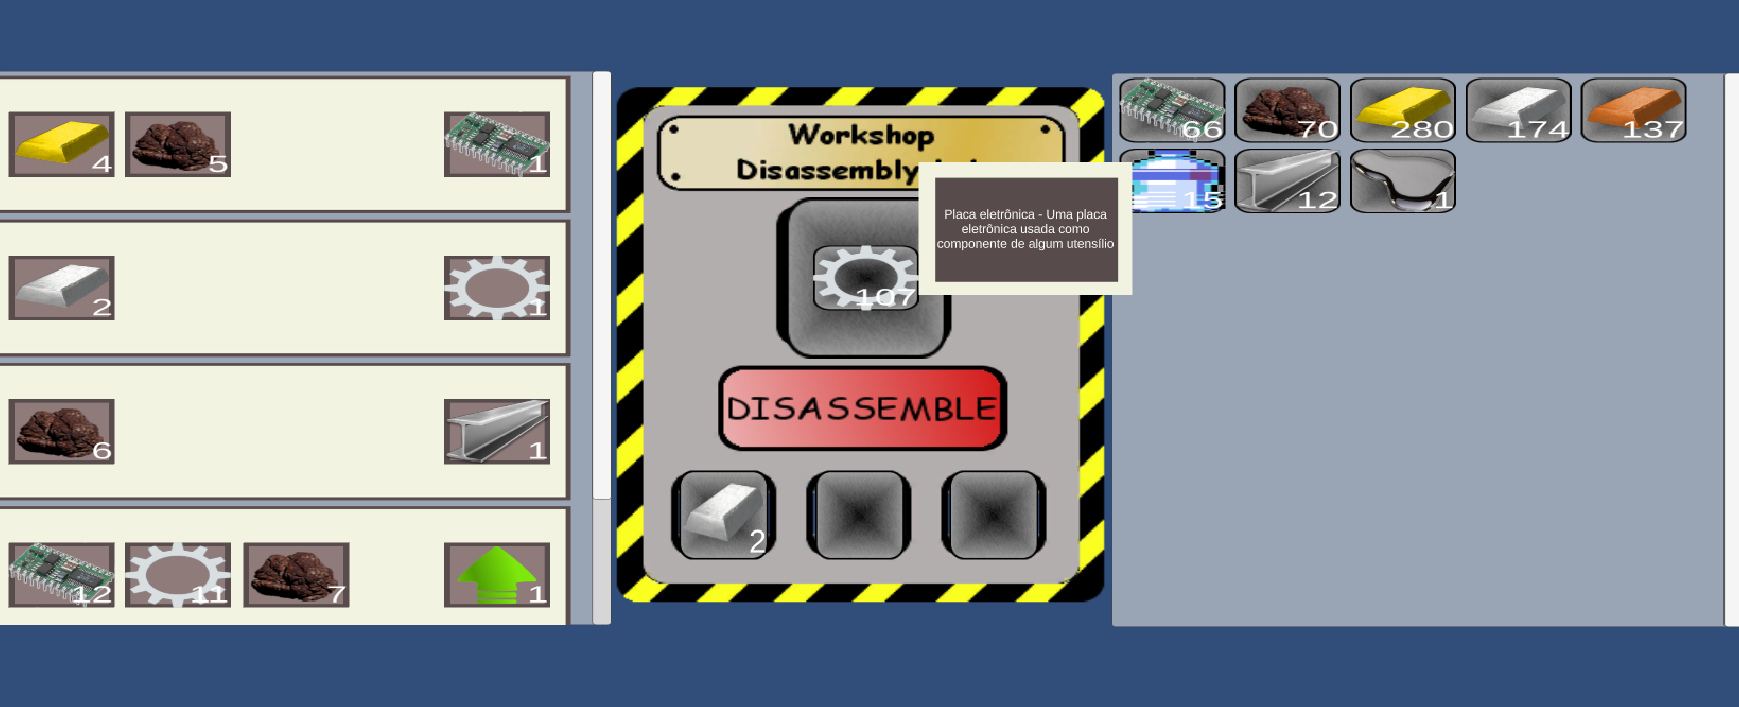
\includegraphics[width=500px]{figuras/disassembly.png}
    \caption{Laboratório de desmontagem - Desmontando um item}
    \label{fig_disassembler}
\end{figure}

\subsection{Laboratório de montagem}
Aplicado os conceitos de Crafting voltados para montar itens complexos ou novas habilidades para o jogador. A partir de receitas (que aponta quais itens são necessários para efetuar a criação), se o jogador oferecer os itens nas as quantidades necessárias, acontece com sucesso a operação.
\begin{figure}[h]
    \centering
    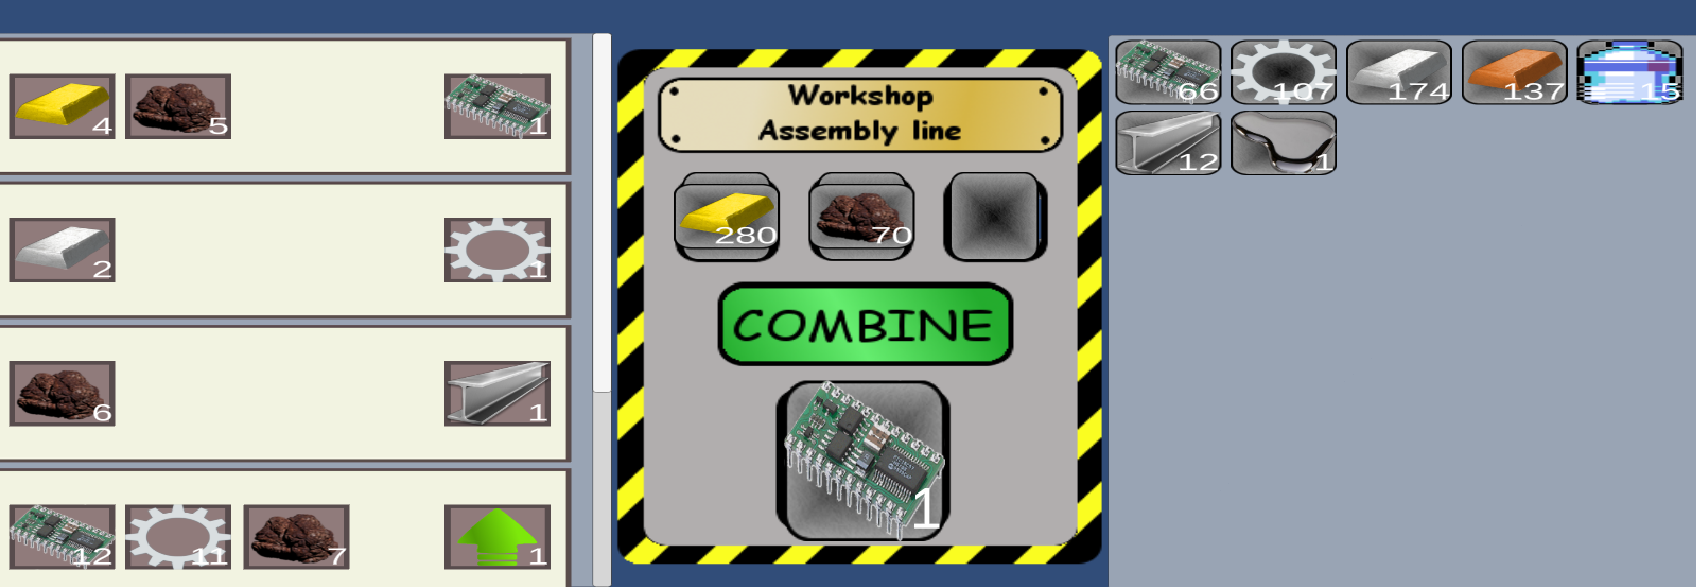
\includegraphics[width=500px]{figuras/assembly.png}
    \caption{Laboratório de montagem}
    \label{fig_assembler}
\end{figure}

\section{Discussão}
%Amarrar os conceitos de IHC com o desenvolvimento do jogo: como as personas foram usadas no desenvolvimento, cenários, análise de tarefas.
A crescente preocupação com questões ambientais é cada vez mais evidente na sociedade contemporânea e desempenha um papel crucial na busca por um futuro sustentável. O jogo em questão aborda especificamente a temática da preservação do meio ambiente, apresentando a organização criminosa Eco-InterCrim como responsável por desastres ambientais decorrentes do descarte inadequado de materiais. Essa abordagem tem o potencial de despertar o interesse dos jogadores e conscientizá-los sobre a importância da destinação correta de resíduos e ações voltadas para a redução do impacto humano no meio ambiente.

Além disso, o jogo transmite uma mensagem positiva, enfatizando que cada pessoa tem o poder de fazer a diferença ao agir em prol da proteção ambiental. O personagem Weee, por exemplo, assume o papel de herói ao frustrar os planos da organização criminosa. Adicionalmente, a mecânica de coleta de itens no jogo pode ser interpretada como uma forma de incentivar a reciclagem e a reutilização de materiais.

Com base nas personas definidas na (Tabela \ref{table:personasTable}), o desenvolvimento do jogo sugere ao jogador, por meio de dicas, a possibilidade de descobrir e aprender detalhes sobre o jogo. Um dos objetivos finais estabelecidos pela Análise Hierárquica de Tarefas (ver imagem \ref{fig_analise_hierarquica_b}) é justamente superar obstáculos, e uma maneira de introduzir dificuldades nesse objetivo é trazer a necessidade das personas de adquirir aprimoramentos para o personagem, outro objetivo final identificado na AHT (ver imagem \ref{fig_analise_hierarquica_c}). Para alcançar esses aprimoramentos, é necessário coletar os itens disponíveis em cada fase do jogo e derrotar os inimigos, que também são objetivos finais. O equilíbrio entre esses objetivos, aliado à proposta de aprendizado do jogo, visa proporcionar desafios para as personas e uma sensação de progresso a cada nova evolução alcançada (ver \ref{cenarios}), juntamente com a possibilidade de repetir as fases para acumular mais itens.

Embora o jogo não tenha a intenção de fornecer soluções concretas para os problemas ambientais, ele pode ser uma ferramenta eficaz para estimular a reflexão sobre a importância da preservação do meio ambiente e a responsabilidade individual em relação a esse tema. Educadores e professores podem utilizar o jogo como recurso em atividades de conscientização e educação ambiental, proporcionando uma abordagem lúdica para tratar de um assunto tão relevante.

Sob a óptica de IHC, What Weee Are se propõe a trazer os seguintes conceitos:

\begin{itemize}
    \item Usabilidade: O jogo deve ser fácil e intuitivo de jogar, com controles simples e fáceis de entender para que o jogador possa se concentrar na jogabilidade e na história do jogo.

    \item Feedback: O jogo deve fornecer feedback ao jogador sobre suas ações. Por exemplo, quando Weee coleta um item ou derrota um inimigo, o jogador deve receber uma notificação ou som para indicar que o objetivo foi alcançado.

    \item Design centrado no usuário: O jogo deve ser projetado pensando nas necessidades e preferências do usuário. Por exemplo, a interface deve ser clara e legível, com tamanho de fonte adequado e cores que não prejudiquem a visibilidade.

    \item Acessibilidade: O jogo deve ser acessível a um público amplo, incluindo pessoas com deficiência visual ou auditiva. Por exemplo, o jogo poderia ter opções de legendas ou opções de áudio para que os jogadores possam escolher a melhor forma de jogar.

    \item Consistência: O jogo deve ser consistente em toda a experiência do usuário, incluindo os controles, a aparência visual e a jogabilidade. Isso ajuda a garantir que o jogador não fique confuso ou frustrado enquanto joga.

    \item Personalização: O jogo poderia incluir opções de personalização, permitindo que os jogadores escolham sua própria aparência para o personagem ou o tipo de som que preferem ouvir.
\end{itemize}

Esses são apenas alguns exemplos de conceitos de Interação Humano-Computador que poderiam ser aplicados ao jogo "What Weee Are".
Inicialmente junto da persona João Pedro, o professor, foi utilizados seus conhecimentos acerca dos problemas causados pelo desperdício de materiais eletrônicos e como poderíamos aborda-los dentro do jogo. Contribuiu com a concepção do Sistema de Crafting (\ref{craft}), como mecânica que iria abordar como é possível reciclar e reatribuir uso a objetos, que antes seriam vistos como lixo, a se tornarem úteis novamente. As personas que iriam jogar o jogo, Natália e Leonardo, foram importante em como elaborar as fases e a dificuldade do jogo a ponto que, alunos de idade de 5 a 12 anos conseguissem prosseguir sem dificuldade, com uma linguagem simples que fosse capaz de apresentar o roteiro sem dificuldade de interpretação. Que fosse desafiador à alunos como Leonardo, que possuem facilidade em mecânicas de jogos, reaproveitando a comunicação simples. 
\par
O jogo foi desenvolvido em paralelo com a análise de tarefas, pois o jogo sofreu de influência de conceitos comumente apresentados em jogos muito conhecidos, plataforma 2D. Como
\begin{itemize}
    \item Super Mario World - Inspirou em como fazer uso de plataformas e dificuldade
    \item Donkey Kong Country - Inspirou em narrativa
    \item Megaman - Inspirou em conceitos de evolução de habilidades do personagem
    \item Minecraft - Inspirou no Sistema de Crafting
\end{itemize}

A partir destes conceitos distintos, a análise de tarefas junta-os em uma experiência com que seja possível fazer uso de forma contínua e fluida enquanto as personas jogam. O Professor João Pedro voltou a participar do processo de desenvolvimento, a fim de ajudar na escolha de quais itens seriam possível construir a partir do sistema de crafting, e quais upgrades estariam presentes em What Weee Are a partir da reciclagem dos materiais. 



\chapter{Considerações Finais}
\label{conclusao}

Neste capítulo, são apresentadas as possibilidades existentes que ainda podem ser exploradas no desenvolvimento do jogo em futuras versões, além de disponibilizar o código-fonte do projeto para que todos possam contribuir.

What Weee Are é um jogo com infinitas possibilidades. A adição de cenários, itens e novos aprimoramentos ao personagem são apenas algumas das opções. O Unity Analytics pode ser uma poderosa ferramenta capaz de propor a implementação de testes A/B durante o jogo, coletar dados a partir de cada teste e realizar estudos com base nas decisões dos jogadores para continuar refinando e melhorando o jogo no futuro.

\section{Trabalhos Futuros}
Em What Weee Are, a expansão do universo é um fato. Os maiores desenvolvimentos neste estágio atual foram a implementação de mecânicas básicas e estruturas que proporcionam justamente a facilidade ao adicionar novos recursos no jogo. A adição de novos itens e receitas basta adicionar novos itens nos arquivos JSON que definem os itens, e a adição de novos diálogos se torna a adição de um novo GameObject do tipo Dialogue. Porém, no futuro, há a possibilidade de levá-lo para dispositivos móveis e também a captação de Analytics (coletar dados de tomada de decisão, tempo de jogo, coleta dos itens, derrota dos inimigos) para servir de insumo ao construir novas fases e também à evolução de aprendizado dos jogadores, conforme o progresso do jogo, por meio da ferramenta robusta oferecida pela própria UNITY, o UNITY ANALYTICS \footnote{Veja mais em: https://unity.com/products/unity-analytics}.

O uso dos dados gerados a partir do \textit{analytics} poderá proporcionar a implementação de testes A/B durante o jogo, para, enfim, analisar a implementação e o resultado de novas abordagens, implementação de modos mais desafiadores e recompensadores aos jogadores. Isso poderá trazer análises sobre as decisões tomadas em pontos-chave do jogo e, assim, projetar melhorias aos cenários e, por fim, proporcionar uma melhor experiência aos jogadores.

What Weee Are é um jogo de código aberto, pronto para receber novas ideias e implementações de desenvolvedores e jogadores que se sintam à vontade para contribuir com a progressão e novos estágios do jogo. O projeto pode ser encontrado aqui: \url{https://github.com/iRitiLopes/WhatWeeAre}


\section{Possibilidades}
\begin{itemize}
    \item Desenvolvimento e teste do jogo educativo "What Weee Are" para avaliar sua eficácia em fornecer informações e conscientização sobre a reciclagem de resíduos eletrônicos e suas consequências para o meio ambiente.
    \item Análise da eficácia dos jogos educativos no contexto dos Objetivos de Desenvolvimento Sustentável da ONU em comparação com outros métodos de conscientização, como palestras e vídeos informativos.
    \item Estudo da importância da cocriação no desenvolvimento de jogos educativos e digitais, e sua influência na aceitação e eficácia desses jogos.
    \item Investigação do uso de ferramentas de análise de dados, como o Unity Analytics, na avaliação do desempenho do jogador e na coleta de feedback do usuário, para melhorar a eficácia do jogo educativo e a experiência do usuário.
    \item Desenvolvimento de uma plataforma de jogos educativos para a conscientização ambiental e sustentabilidade, permitindo que outros desenvolvedores contribuam com jogos e conteúdos educacionais.
    \item Avaliação do impacto social e ambiental dos jogos educativos na conscientização e mudança de comportamento dos jogadores em relação à sustentabilidade e reciclagem de resíduos eletrônicos.
    \item Exploração de outras tecnologias, como realidade virtual ou aumentada, para aprimorar a experiência do jogador e aumentar o impacto dos jogos educativos no público-alvo.
    \item Investigação de estratégias para incentivar o uso de jogos educativos em escolas e programas educacionais formais para apoiar a conscientização e educação em sustentabilidade e desenvolvimento sustentável.
    \item Comparação da eficácia dos jogos educativos em diferentes contextos, como faixa etária, nível educacional, contexto cultural e socioeconômico, e como essa informação pode ser usada para aprimorar o design e a disseminação dos jogos educativos.
\end{itemize}
% 9)  Referências
%
% IMPORTANTE!! Projeto para submeter ao comite de ética PRAZO INICIO DE JUNHO
%

% ----------------------------------------------------------
% ELEMENTOS PÓS-TEXTUAIS
% ----------------------------------------------------------
\postextual
% ----------------------------------------------------------

% ----------------------------------------------------------
% Referências bibliográficas
% ----------------------------------------------------------
\bibliography{PGC.bib}


%\chapter{Anexos}
\begin{figure}[h]
    \centering % este comando é usado para centralizar a figura
    \caption{Fluxograma de Telas}
	\label{fig_fluxo}
	\includegraphics[width=10cm]{figuras/fluxo.png}\\
\end{figure}
%---------------------------------------------------------------------
% INDICE REMISSIVO
%---------------------------------------------------------------------
\phantompart
\printindex


%---------------------------------------------------------------------

\end{document}
